%==============================================================================
%  Spectral top-down split recovery on imbalanced phylogenetic trees  --  V.10
%
%  Thin master: preamble, \maketitle, the \input list, bibliography and appendix
%  switches.  All prose lives in sections/, whose filenames give the reading order.
%==============================================================================
\documentclass[11pt]{article}
\usepackage[margin=1in]{geometry}
\usepackage{amsmath,amssymb,amsthm,mathtools}
\usepackage{enumitem}
\usepackage{booktabs}
\usepackage{algorithm}
\usepackage[noend]{algpseudocode}
\usepackage{graphicx}
\usepackage{subcaption}
\usepackage{xcolor}
\usepackage{tikz}
\usetikzlibrary{positioning, shapes.geometric, arrows.meta, calc, fit, backgrounds}
\usepackage{hyperref,cleveref}
\crefname{assumption}{Assumption}{Assumptions}
\Crefname{assumption}{Assumption}{Assumptions}
\crefname{condition}{Condition}{Conditions}
\Crefname{condition}{Condition}{Conditions}

% Self-contained: every \includegraphics resolves inside v10/figures/.  Do NOT re-add
% `{../}` -- it resolved figures outside this tree and broke an Overleaf upload.
\graphicspath{{figures/}{./}}
\bibliographystyle{plain}

%------------------------------ theorem environments --------------------------
\theoremstyle{plain}
\newtheorem{theorem}{Theorem}
\newtheorem{lemma}{Lemma}
\newtheorem{proposition}{Proposition}
\newtheorem{corollary}{Corollary}

\theoremstyle{definition}
\newtheorem{definition}{Definition}
\newtheorem{assumption}{Assumption}
\renewcommand{\theassumption}{A\arabic{assumption}}   % => A1, A2, ...
% C1 is on its own counter so A1/A2 count only the two modelling hypotheses; it is a
% quantitative inequality, not an assumption about the data.  Label: asm:margin.
\newtheorem{condition}{Condition}
\renewcommand{\thecondition}{C\arabic{condition}}     % => C1

\theoremstyle{remark}
\newtheorem{remark}{Remark}

%------------------------------ notation shortcuts ----------------------------
% \Sin always carries a superscript: \Sin^{\min} is the weakest within-block
% similarity of def:cfbm.  \Smax is the largest off-diagonal entry, max_{i!=j} S_ij.
% The cross-block baseline has one name, \bze; \Sout is retired with it.
\newcommand{\Sin}{S_{\mathrm{in}}}
\newcommand{\Smax}{S_{\max}}
\newcommand{\bze}{\beta_0}
\newcommand{\Dlam}{\Delta\lambda}
\newcommand{\vv}{v^{(2)}}
\newcommand{\vvh}{\hat v^{(2)}}
\newcommand{\EL}{E_{L}}
\newcommand{\ES}{E_{S}}
\newcommand{\ED}{E_{D}}
\newcommand{\coh}{\mu(U)}
% Fiedler sign partition: \Pisp{S} population, \Pisp{\hat S} empirical.  Introduced
% in §2 at thm:stdr-split.  A clan pair of the tree by thm:stdr-split, unconditionally.
\newcommand{\Pisp}[1]{\Pi(#1)}
\newcommand{\rhotil}{\tilde\rho(\eta)}
\newcommand{\norm}[1]{\left\lVert #1 \right\rVert}
\newcommand{\opnorm}[1]{\norm{#1}_{2}}
\newcommand{\hp}{with high probability}
\newcommand{\R}{\mathbb{R}}
\newcommand{\1}{\mathbf{1}}
\newcommand{\E}{\mathbb{E}}
\newcommand{\Prob}{\mathbb{P}}

\title{Spectral Tree Inference from Incomplete Matrices: Fiedler Vector Bounds under Sub-sampling}
\author{Itay Gonnen}
\date{}

\begin{document}
\maketitle

% Abstract.  One paragraph, one claim: a sampling rate of order log m / m suffices for
% the sub-sampled Fiedler split to reproduce the full-data split, and the imbalance eta
% is the parameter that governs the cost.
\begin{abstract}
Top-down reconstruction of latent binary phylogenetic trees is fundamentally bottlenecked by the $\Theta(m^2)$ cost of computing pairwise similarities across $m$ leaves. While observing only a sparse, Bernoulli-sampled subset of entries offers a computational workaround, real-world tree imbalance severely degrades the spectral signal, rendering standard balanced-cluster recovery guarantees inadequate. 
In this work, we frame spectral tree inference as an eigenvector perturbation problem within the matrix-completion regime, showing that the split obtained from the full similarity matrix of an imbalanced latent tree is recovered exactly from the sign pattern of the empirical Fiedler vector computed on a sparse sample. That split is an edge cut of the tree for any topology.

Our primary contribution is a sharp finite-sample guarantee proving that a sampling rate of $p = \Theta(\log m / m)$ suffices for exact recovery of that split at a fixed imbalance. By utilizing a coordinate-wise Neumann-series expansion rather than a standard Davis-Kahan $\ell_2$ transfer, we eliminate a spurious $\sqrt{m}$ factor in the entry-wise error bound. 
Furthermore, we identify the imbalance ratio $\eta$ as the governing topological parameter and prove it dictates recovery through two distinct failure mechanisms: artificially inflating subspace coherence (rendering recovery statistically unaffordable) and eroding the spectral gap (rendering recovery structurally impossible). 
This yields an explicit sample complexity dependence of $(1+\eta)^3$. Simulations on closed-form block models and Kingman coalescent trees with JC69 sequence evolution validate the predicted $\Theta(\log m / m)$ scaling and the isolated degradation mechanics of topological imbalance.
\end{abstract}


%==============================================================================
%  Main text
%==============================================================================
% §1 Introduction (Related Work folded in).  Point: the top split of a top-down
% spectral method is the expensive call, and sub-sampling it is not routine -- coherence,
% tree imbalance and the gap between 2-norm and entry-wise control all bite.
\section{Introduction}\label{sec:intro}

A latent tree graphical model relates $m$ observed leaves through unobserved
internal nodes, and the inference problem is to recover the topology from leaf
data alone \cite{aizenbud2023spectral, semple2003phylogenetics}. Phylogenetics is
the canonical instance and supplies our vocabulary: the leaves are extant
organisms, the internal nodes their extinct ancestors, the data aligned
sequences. Distance-, likelihood- and spectral-based reconstruction are all well
developed \cite{saitou1987neighbor, erdos1999logs, jaffe2021spectral,
mossel2005learning}, but datasets now reach tens of thousands of leaves, and the
accurate methods are the slow ones.

That pressure produced the top-down spectral family, which is spectral clustering
run on a phylogeny. Build a similarity matrix $S$ over the leaves, form the
Laplacian $L=D-S$, split the leaf set by the sign pattern of the Fiedler vector
of $L$, recurse on each side, and merge \cite{aizenbud2023spectral,
vonluxburg2007tutorial, fiedler1975property}. The split is provably consistent:
the two sides are the two halves of a single edge cut --- a \emph{split} of the tree
\cite{wilkinson2007clades} --- which is what keeps the merge tractable. Both the
error and the cost of the recursion land on the top split, since no parent call
corrects it and it is the only call that sees all $m$ leaves. Every entry of $S$
is a sequence-pair estimate over a length-$\ell$ alignment rather than a lookup,
so that one call costs $\Theta(m^2)$ estimator evaluations --- the cost
divide-and-conquer exists to avoid.

This paper asks what happens to the spectrum when that cost is not paid. Compute
only a random $p$-fraction of the pairs, reweight the survivors by $1/p$, and
take the Fiedler vector of the incomplete matrix, in the manner of low-rank
matrix completion \cite{candes2008exact, candes2009power, candes2009matrix,
recht2011simpler, keshavan2010matrix, bhojanapalli2014universal}. Does its sign
pattern still recover the split, and how small can $p$ be? There is reason to
expect an answer well below $1$: under a molecular clock the population matrix
has exactly two blocks and the Fiedler vector is constant on each clade
(\Cref{sec:assumptions}), so the signal being sampled is extremely concentrated.

Two things keep this from being routine. What decides recoverability from a
random subset is how spread the leading subspace is across coordinates, not how
large the matrix is \cite{chen2014completing}; and guarantees for recursive
spectral bipartitioning are stated for clusters of comparable size
\cite{Balakrishnan2011clustering, qinrohe2013regularized}, whereas real
phylogenies are markedly more imbalanced than standard null models predict
\cite{blum2006which, yule1925mathematical, kingman1982coalescent,
steel2001properties, aldous2001stochastic}. Imbalance pushes both governing
quantities the wrong way: it concentrates the split signal onto the smaller clade,
raising the sampling cost, and it shrinks the eigenvalue gap that isolates the
Fiedler vector, degrading the signal itself. The two failures are distinct ---
one leaves the eigenvector informative but unaffordable to sample, the other
leaves nothing worth sampling --- so pooling them shows one curve where there are
two mechanisms.

Recovering a split from a sign pattern is a claim about \emph{every} coordinate
of an eigenvector, whereas classical perturbation theory controls only its
Euclidean norm \cite{davis1970rotation};
passing between the two charges every node as though it were the worst one, which
here decides whether a guarantee is satisfiable at all. We therefore work
coordinate-wise \cite{eldridge2017unperturbed, fan2018eigenvector,
abbe2020entrywise, tropp2012userfriendly}.

Our contributions are:
\begin{itemize}
\item We make the imbalance ratio $\eta$ the single parameter through which tree
shape reaches the linear algebra, and express both governing spectral quantities
in it: the subspace coherence in closed form, and a lower bound on the Fiedler
gap (\Cref{sec:bridging}).

\item We prove that a sampling rate of order $\log m/m$ suffices, at fixed
imbalance, for the sign pattern of the empirical Fiedler vector to reproduce the
full-data split exactly \hp, with an explicit cubic dependence on $\eta$
(\Cref{sec:main}). 

\item The proof works coordinate-wise rather than in Euclidean norm, through a
Neumann expansion and a per-node Bernstein bound (\Cref{sec:outline}); on this
model the Euclidean route costs a further factor of $m$ in the required rate.

\item We test the rate in simulation, scoring each sub-sampled split against the one the full
matrix returns \cite{strehlghosh2002cluster, fortunato2010community} and stratifying by imbalance
rather than pooling (\Cref{sec:empirical}).
\end{itemize}

\Cref{sec:background} fixes the objects: the tree, the substitution model, the similarity graph
and its Fiedler vector, and the result that the Fiedler split is always a split of the tree.
\Cref{sec:problem} builds the STDR recursion on that result and states the problem --- the
quadratic cost of its top-level call, the sampling scheme that answers it, and the entry-wise
criterion that decides whether the sampled split is the right one. \Cref{sec:assumptions} collects every hypothesis the
analysis carries: the molecular clock, the block model it induces, the imbalance $\eta$ and the
margin $\rho$. \Cref{sec:main} states the rate. \Cref{sec:bridging} then routes tree shape into
the spectrum through $\eta$: it identifies which split the population Fiedler vector returns and
bounds the two failure modes. \Cref{sec:outline} assembles the proof and \Cref{sec:empirical}
tests the rate.

Related work is woven into the argument above rather than sectioned off.
        % §1  Introduction (incl. Related Work as §1.1)
% §2 Background.  Delivers the objects the paper is about: tree, substitution model, similarity
% and distance, the similarity graph and its Fiedler vector, clades, thm:stdr-split.  No modelling
% hypothesis is made here: the algorithm and the sampling scheme are §3, every assumption of the
% analysis is §4.
\section{Background}\label{sec:background}

This section presents the objects the paper works with and the algorithm it accelerates.
\Cref{sec:bg-model} sets the tree and the substitution process running on it,
\Cref{sec:bg-similarity} the similarity and distance matrices they induce on the terminal nodes,
the graph those matrices define, the bipartitions a tree admits, and the result that the Fiedler
vector always returns one of them.
\Cref{sec:problem} builds the reconstruction algorithm on that result and states the problem this
paper solves.

\subsection{The generative model}\label{sec:bg-model}

\subsubsection*{Tree topology}

Let $\mathcal{T} = (V, E)$ be a rooted binary phylogenetic tree whose vertex set
$V = \mathcal{X} \cup \mathcal{H}$ consists of $m$ observed terminal nodes
$\mathcal{X} = \{x_1, \dots, x_m\}$ and $m-1$ unobserved internal nodes
$\mathcal{H} = \{h_1, \dots, h_{m-1}\}$.  We denote by 
$r \in \mathcal{H}$ the root of the tree. 
In a binary tree, all terminal nodes have a single neighbor,  the internal nodes except the root have three neighbors and the root has two neighbors. In phylogenetics, the terminal nodes represent extant organisms, while the internal nodes represent their common ancestors.

Every edge $e = (h, h') \in E$ is assigned a \emph{branch length} $t_e \ge 0$, which is a measure of the evolutionary divergence between the two adjacent nodes it joins. 
We represented branch lengths through
absolute node heights: each node $h$ is assigned a height $\tau_h \ge 0$ measured upward from the
terminal nodes, such that $t_e = t_{(h,h')} = |\tau_h - \tau_{h'}|$.


\begin{definition}[Most recent common ancestor]\label{def:mrca} For two termianl nodes $x_i, x_j$ of $\mathcal{X}$, the \emph{most recent common ancestor} $\mathrm{MRCA}(x_i,x_j)$ is the node with the smallest value $\tau$ among the common ancestors of $x_i$ and $x_j$ \cite{semple2003phylogenetics}. We denote the height of this most recent common ancestor by $\tau_{ij}$.
\end{definition}
\noindent For a pair of terminal nodes $x_i, x_j$, let $\mathrm{path}(x_i,x_j)$ denote the unique sequence of edges connecting them in $\mathcal{T}$. We define the total length of the path joining them as
\begin{equation}\label{eq:path_length}
d_{ij} := \sum_{e \in \mathrm{path}(x_i,x_j)} t_e .
\end{equation}

\Cref{fig:tree_topology} illustrates a rooted tree with $m = 7$ terminal nodes.



\begin{figure}[t]
\centering
\footnotesize
\tikzset{
  inode/.style={circle, draw, fill=black!8, minimum size=6.6mm, inner sep=0pt,
                font=\tiny},
  lfN/.style={circle, draw, fill=black!8, minimum size=6.6mm, inner sep=0pt,
              font=\tiny},
  % endpoint of a highlighted path: contour in that path's colour
  lfblue/.style={lfN, draw=blue!70!black, line width=1.1pt},
  lforng/.style={lfN, draw=orange!85!black, line width=1.1pt},
  lfA/.style={circle, draw, fill=blue!22, minimum size=6.6mm, inner sep=0pt,
              font=\tiny},
  lfB/.style={circle, draw, fill=red!22, minimum size=6.6mm, inner sep=0pt,
              font=\tiny},
  br/.style={thick, black!65},
  hl/.style={line width=1.6pt, blue!70!black},
  hlr/.style={line width=1.6pt, orange!85!black},
  guide/.style={densely dotted, black!45},
  cutB/.style={line width=1pt, green!45!black, dash pattern=on 3pt off 2pt},
}

%----------------------------------------------------------------- panel (a)
\begin{subfigure}[t]{0.49\textwidth}
\centering
\begin{tikzpicture}[x=1cm, y=1.15cm]
  % leaves -- neutral fill: this panel is about heights, not clades
  \node[lfblue] (x1) at (-2.35,0) {$x_1$};
  \node[lfblue] (x2) at (-1.55,0) {$x_2$};
  \node[lforng] (x3) at (-0.75,0) {$x_3$};
  \node[lfN]    (x4) at ( 0.30,0) {$x_4$};
  \node[lforng] (x5) at ( 1.10,0) {$x_5$};
  \node[lfN] (x6) at ( 1.90,0) {$x_6$};
  \node[lfN] (x7) at ( 2.70,0) {$x_7$};
  % internal; the two MRCAs carry the colour of their path
  \node[inode, fill=blue!30]   (u)  at (-1.95,0.80) {};
  \node[inode]                 (hA) at (-1.35,1.80) {$h_1$};
  \node[inode]                 (w)  at ( 0.70,0.80) {};
  \node[inode]                 (z)  at ( 2.30,0.80) {};
  \node[inode]                 (hB) at ( 1.50,1.35) {$h_2$};
  \node[inode, fill=orange!35] (r)  at ( 0.10,2.45) {$r$};
  % branches
  \draw[br] (r)--(hA); \draw[br] (r)--(hB);
  \draw[br] (hA)--(u); \draw[br] (hA)--(x3);
  \draw[br] (u)--(x1); \draw[br] (u)--(x2);
  \draw[br] (hB)--(w); \draw[br] (hB)--(z);
  \draw[br] (w)--(x4); \draw[br] (w)--(x5);
  \draw[br] (z)--(x6); \draw[br] (z)--(x7);
  % two edge-disjoint paths: within-block x1 -- u -- x2, cross-block x3 -- r -- x5
  \draw[hlr] (x3)--(hA)--(r)--(hB)--(w)--(x5);
  \draw[hl]  (x1)--(u)--(x2);
  % height axis
  \draw[black!55, -{Latex[length=1.4mm]}] (-3.15,-0.05) -- (-3.15,2.85)
        node[above, font=\scriptsize, black!55] {$\tau$};
  \foreach \y/\lbl in {0/$0$, 0.80/$\tau_{12}$, 2.45/$\tau_r$}{
     \draw[black!55] (-3.25,\y) -- (-3.05,\y);
     \node[left=0pt, font=\scriptsize, black!70] at (-3.25,\y) {\lbl};
  }
  \draw[guide] (-3.05,0.80) -- (u);
  \draw[guide] (-3.05,2.45) -- (r);
  \draw[guide] (-3.05,0) -- (x1);
  % annotations
  \node[font=\scriptsize, blue!70!black] at (-1.95,-0.62) {$\mathrm{MRCA}(x_1,x_2)$};
  \node[font=\scriptsize, orange!75!black, align=left, anchor=west] at (0.45,2.82)
        {$\mathrm{MRCA}(x_3,x_5)=r$\\[-1pt] so $\tau_{35}=\tau_r$};
\end{tikzpicture}
\subcaption{Heights and coalescence}\label{fig:topology-heights}
\end{subfigure}
\hfill
%----------------------------------------------------------------- panel (b)
\begin{subfigure}[t]{0.49\textwidth}
\centering
\begin{tikzpicture}[x=1cm, y=1.15cm]
  \node[lfB] (x1) at (-2.35,0) {$x_1$};
  \node[lfB] (x2) at (-1.55,0) {$x_2$};
  \node[lfB] (x3) at (-0.75,0) {$x_3$};
  \node[lfB] (x4) at ( 0.30,0) {$x_4$};
  \node[lfB] (x5) at ( 1.10,0) {$x_5$};
  \node[lfA] (x6) at ( 1.90,0) {$x_6$};
  \node[lfA] (x7) at ( 2.70,0) {$x_7$};
  \node[inode] (u)  at (-1.95,0.80) {};
  \node[inode] (hA) at (-1.35,1.80) {};
  \node[inode] (w)  at ( 0.70,0.80) {};
  \node[inode] (z)  at ( 2.30,0.80) {};
  \node[inode] (hB) at ( 1.50,1.35) {};
  \node[inode] (r)  at ( 0.10,2.45) {$r$};
  \draw[br] (r)--(hA); \draw[br] (r)--(hB);
  \draw[br] (hA)--(u); \draw[br] (hA)--(x3);
  \draw[br] (u)--(x1); \draw[br] (u)--(x2);
  \draw[br] (hB)--(w); \draw[br] (hB)--(z);
  \draw[br] (w)--(x4); \draw[br] (w)--(x5);
  \draw[br] (z)--(x6); \draw[br] (z)--(x7);
  % one edge cut, above z: C1 = {x6,x7}, C2 = everything else
  \coordinate (m1) at ($(hB)!0.5!(z)$);
  \draw[cutB] ($(m1)!0.45cm!90:(z)$) -- ($(m1)!0.45cm!-90:(z)$);
  \node[font=\scriptsize, green!45!black, align=left, anchor=west] at (2.95,1.35)
        {one edge\\[-1pt] cut};
  \node[font=\scriptsize, green!45!black] at (2.30,-0.62) {$C_1$};
  \node[font=\scriptsize, green!45!black] at (-0.55,-0.62) {$C_2$};
\end{tikzpicture}
\subcaption{Clades and edge cuts}\label{fig:topology-clades}
\end{subfigure}

\caption{A tree with $m=7$ terminal nodes. \textbf{(a)} Node heights $\tau$ increase toward the root, and $\tau_{ij}$ is the height of $\mathrm{MRCA}(x_i,x_j)$ (see \Cref{def:mrca}). The blue path joins a pair that coalesces early; the orange path joins a pair whose most recent common ancestor is the root, so $\tau_{35}=\tau_r$. \textbf{(b)} Removing a single edge splits the terminal nodes in two (\Cref{def:clade}); the cut shown gives $C_1=\{x_6,x_7\}$ and $C_2=\{x_1,\dots,x_5\}$.}
\label{fig:tree_topology}
\end{figure}

\subsubsection*{The substitution process}

We assume that the observed sequences are generated according to the common model of sequence evolution, described by a Markov process along the edges of the single latent tree $\mathcal{T}$ (see, e.g.,~\cite[Chapter 1]{yang2014molecular}). 
Specifically, at each node $h$ in the tree, there is an associated discrete random variable $X_h$ over the alphabet $\{1, \ldots, q\}$. For example, in the common DNA setting, the support of each node consists of $q=4$ characters representing the basic nucleotides $\{A,C,G,T\}$.

In addition, every edge $e(h, h')$ connecting a pair of adjacent nodes is equipped with transition matrices of size $q \times q$. The sequence generative process begins at the root, where its state is drawn according to some initial distribution over $\{1, \ldots, q\}$. Then, for any parent node $h' \in \mathcal{H}$ connected by an edge to a child node $h \in \mathcal{H}$, the transition matrix $P(h \mid h') \in \mathbb{R}^{q \times q}$ is 
\begin{equation}
    P(h \mid h')_{ba} = \Prob(X_{h} = b \mid X_{h'} = a), \qquad a, b \in \{1, \ldots, q\}.
    \label{eq:P_h_htag}
\end{equation}
This process propagates from the root to the terminal nodes. The observed sequences of length $\ell$ for each of the terminal nodes are generated by this process, independently for each location in the sequence.


\paragraph{The GTR model for transition matrices.}
We assume the GTR model for the transition matrices. 
Under this model, the sequences mutate along the edges of the tree according to a continuous-time Markov process, with a rate matrix $Q\in \mathbb{R}^{q\times q}$ that satisfies the following four properties:


\begin{enumerate}[label=(\roman*), leftmargin=2.2em, itemsep=1pt, topsep=3pt]
\item $Q_{ij}\ge0$ for $i\ne j$,
\item $\sum_j Q_{ij}=0$ for all $i$;
\item there is a stationary distribution $\pi>0$ with $\pi Q=0$; and
\item $\mathrm{diag}(\pi)\,Q$ is symmetric.
\end{enumerate}
Conditions (i)--(ii) define $Q$ as the \emph{infinitesimal generator} of a continuous-time Markov chain. This means $Q$ generates the transition probability matrix for any time $t\ge0$ via the matrix exponential $\exp(Qt)$. Specifically, its off-diagonal entries are the instantaneous rates at which one character is replaced by another, and its rows sum to zero to ensure that $\exp(Qt)$ is a valid stochastic matrix. Condition (iii) says the character frequencies $\pi$ are left unchanged by the process, and (iv) makes it \emph{reversible} --- a path observed forwards in time and the same path observed backwards have the same probability, $\pi_a\,[\exp(Qt)]_{ab}=\pi_b\,[\exp(Qt)]_{ba}$. Together (i)--(iv) imply that all eigenvalues of $Q$ are non-positive, and hence that $\mathrm{tr}(Q)<0$.

For two \emph{adjacent} nodes $h,h'$, the substitution matrix over the branch joining them is equal to the matrix exponential of the generator scaled by the branch length,
\begin{equation}\label{eq:transition_matrix}
P(h \mid h') = \exp\bigl(Q t_{(h,h')}\bigr),
\end{equation}

\subsection{Similarity, distance and the similarity graph}\label{sec:bg-similarity}

The substitution model provides a measure of similarity between every pair of nodes in the tree. e first define this pairwise similarity function, and subsequently construct the similarity matrix over the observed terminal nodes.

\begin{definition}[Pairwise similarity function]\label{def:similarity}
Let $\det(\cdot)$ denote the matrix determinant. The pairwise similarity function between any two nodes $h_i$ and $h_j$ is defined based on the determinants of their transition matrices:
\begin{equation}\label{eq:similarity_def}
   S(h_i, h_j) := \sqrt{\det(P(h_i \mid h_j))\,\det(P(h_j \mid h_i))},
   \qquad S(h_i,h_i) = 1 .
\end{equation}
\end{definition}

Because the determinant is a multiplicative function and the transition matrices $P$ , this similarity measure is also multiplicative along the edges of the tree \cite{aizenbud2023spectral}. Under  the GTR model, the transition matrix between two nodes separated by evolutionary distance $d_{ij}$ is $P(x_i \mid x_j) = \exp(Q d_{ij})$. This yields the closed-form expression for any two terminal nodes $x_i$ and $x_j$:
\begin{equation}\label{eq:similarity_gtr}
   S(x_i,x_j) = \exp\bigl(\mathrm{tr}(Q)\,d_{ij}\bigr),
\end{equation}
with $d_{ij}$ representing the path length defined in Eq. \eqref{eq:path_length}. Since the GTR rate matrix satisfies $\mathrm{tr}(Q)<0$, the similarity decays exponentially with respect to the evolutionary distance: nodes whose most recent common ancestor is recent are highly similar, and this similarity decays geometrically as that ancestor recedes into the past.

Next, we use this function to construct the matrix representation for the observed data.

\begin{definition}[Similarity matrix and similarity graph]\label{def:simgraph}
The \emph{similarity graph} $G$ is the complete weighted graph whose vertices are the $m$ terminal nodes of $\mathcal{T}$ and whose edge $(x_i,x_j)$ carries weight $S(x_i,x_j)$ \cite{aizenbud2023spectral}. Its weighted adjacency matrix is the \emph{similarity matrix} $S \in \mathbb{R}^{m \times m}$, which consists of the pairwise similarities over the terminal nodes. The entries of the matrix $S$ are explicitly mapped as:
\begin{equation}
    S_{ij} := S(x_i, x_j),
\end{equation}
yielding a symmetric matrix with a unit diagonal ($S_{ii}=1$ for all $i$).
\end{definition}

Next, we define the Laplacian and Fiedler vector of $G$.

\begin{definition}[Laplacian and Fiedler vector]\label{def:fiedler}
The \emph{combinatorial Laplacian} of the similarity graph is $L := D - S$, where $D$ is diagonal
with $D_{ii} = \sum_j S_{ij}$ \cite{aizenbud2023spectral}. Let 
$0 = \lambda_1 < \lambda_2 \le \lambda_3 \le \dots \le \lambda_m$ denote the Laplacian's eigenvalues. The
\emph{Fiedler vector} $\vv$ is a unit eigenvector corresponding to the second-smallest eigenvalue
$\lambda_2$ \cite{fiedler1975property, vonluxburg2007tutorial}.
\end{definition}



To relate the Fiedler vector $\vv$ to the tree topology, we name the bipartitions of
$\mathcal{X}$ that $\mathcal{T}$ admits.

\begin{definition}[Clade; split]\label{def:clade}
A \emph{clade} of $\mathcal{T}$ is a node together with all of its descendants, identified with
the set of terminal nodes that descend from it \cite{wilkinson2007clades}. Removing a single
edge of $\mathcal{T}$ cuts $\mathcal{X}$ into two parts, a \emph{split} of $\mathcal{T}$
\cite{aizenbud2023spectral}; the part away from the root is a clade, and at the root both parts
are.
\end{definition}

\noindent The splits of $\mathcal{T}$ are therefore its edges, one apiece.
\Cref{fig:topology-clades} illustrates a single cut.


\noindent A candidate bipartition is a split of $\mathcal{T}$ exactly when the block of
similarities it cuts collapses to rank one {\cite[Lem.~3.1]{jaffe2021spectral}}, which is the
precise sense in which the topology of $\mathcal{T}$ is embedded in the structure of $S$. With the
terminal nodes ordered along the split as in \Cref{sec:bg-model}, the within-block pairs occupy
the two diagonal blocks of $S$ and the cross-block pairs its off-diagonal block.



The following theorem states that thresholding the Fiedler vector of the similarity graph cuts a single edge of $\mathcal{T}$.

\begin{theorem}[Consistency of the Fiedler split, {\cite[Thm.~4.2]{aizenbud2023spectral}}]\label{thm:stdr-split}
Let $G$ be the similarity graph of a binary tree $\mathcal{T}$ and let $v$ be the Fiedler vector of
$G$. Partition the terminal nodes by the sign pattern of $v$,
\begin{equation}\label{eq:sign_rule}
   C_1=\{i:\;v_i\ge0\},\qquad C_2=\{j:\;v_j<0\}.
\end{equation}
Then $(C_1,C_2)$ is a split of $\mathcal{T}$.
\end{theorem}

\noindent \Cref{thm:stdr-split} makes no assumption on the tree topology or the substitution
parameters, and it is the property that underlies the divide-and-conquer algorithm presented in
\Cref{sec:problem}. We denote by $\Pisp{S}$ the bipartition
\eqref{eq:sign_rule} of the Fiedler vector of $L=D-S$.

          % §2  Background and the STDR algorithm (sec:background)
% §3 Problem definition.  One continuous argument: the STDR recursion, the Theta(m^2) cost of its
% top-level call, the Bernoulli(p) observation model that answers that cost, and the entry-wise
% criterion eq:entrywise that every bound in the paper is measured against.  No subsections --
% the section is one argument and headings would restart it.
\section{Problem definition}\label{sec:problem}

Because the Fiedler split of the full similarity matrix is always a split of $\mathcal{T}$
(\Cref{thm:stdr-split}), tree reconstruction becomes a divide-and-conquer recursion. Spectral
Top-Down Reconstruction (STDR) \cite{aizenbud2023spectral} forms the similarity matrix over the
current node set, splits it by the sign pattern of the Fiedler vector, solves each side
independently by any accurate reconstruction method once the subproblem is small enough, and merges
the two subtrees along the recovered edge (\Cref{alg:stdr}).

\begin{algorithm}[t]
\caption{Spectral Top-Down Reconstruction (STDR) for Latent Tree Models. The algorithm recursively partitions terminal nodes using the Fiedler vector of the similarity graph until the subset size falls below $m_0$. A base method recovers the small subtrees, which are then deterministically merged by identifying optimal placeholder edges via singular vectors of the cross-similarity matrix \cite{aizenbud2023spectral}.}


\label{alg:stdr}
\begin{algorithmic}[1]
\State \textbf{Input:} $\mathcal{X}$, a set of terminal nodes with associated sequence data of length $\ell$; $m_0$, the maximum partition size for base reconstruction.
\State \textbf{Output:} $\mathcal{T}$, a rooted binary latent tree spanning the terminal nodes $\mathcal{X}$.
\Procedure{STDR}{$\mathcal{X}$}
  \If{$|\mathcal{X}| \le m_0$}
    \State \Return $\textsc{BaseReconstruct}(\mathcal{X})$
           \Comment{any accurate method; superlinear in $|\mathcal{X}|$}
  \EndIf
  \State $S \gets \bigl[\,S(x_i,x_j)\,\bigr]_{x_i,x_j \in \mathcal{X}}$
         \Comment{$\Theta(|\mathcal{X}|^2)$ pairwise estimates}
  \State $L \gets D - S$ \Comment{$D_{ii}=\sum_j S_{ij}$, \Cref{def:fiedler}}
  \State $v \gets$ eigenvector of $L$ at $\lambda_2$ \Comment{the Fiedler vector}
  \State $C_1 \gets \{x_i : v_i \ge 0\}$, \quad $C_2 \gets \{x_j : v_j < 0\}$
         \Comment{a split of $\mathcal{T}$, \Cref{thm:stdr-split}}
  \State $\mathcal{T}_1 \gets \textsc{STDR}(C_1)$, \quad
         $\mathcal{T}_2 \gets \textsc{STDR}(C_2)$
  \State \Return $\textsc{Merge}(\mathcal{T}_1, \mathcal{T}_2, S(C_1, C_2))$
         \Comment{join the two subtrees at recovered placeholder edges}
\EndProcedure
\end{algorithmic}
\end{algorithm}

The recursion is attractive because the expensive part of tree reconstruction is superlinear in the
number of terminal nodes, so cutting the problem in half repeatedly reduces the total work sharply,
while \Cref{thm:stdr-split} guarantees that each cut is a genuine split and the merge is therefore
well-posed \cite{aizenbud2023spectral}.

The top-level call of \Cref{alg:stdr} is the one that governs both the error and the cost. It is the
only call that sees all $m$ terminal nodes, and no parent call corrects it: a wrong split at the
root cannot be repaired further down. It is also where the similarity matrix is largest.

Forming the full matrix at the top level therefore costs
\begin{equation}\label{eq:cost}
   \binom{m}{2} = \Theta(m^2) \ \text{pairwise estimates},
   \qquad \Theta(m^2\ell) \ \text{character comparisons},
\end{equation}
which for $m \sim 10^5$ terminal nodes is on the order of $10^{10}$ pairwise estimates before the
recursion has taken a single step. The quadratic term is exactly the cost that divide-and-conquer
was introduced to avoid, and it is paid in full at the root.

This raises the question the paper answers: can the top-down split be computed at almost linear
cost, with a guarantee that it is still the same split the full matrix would have returned?

Our answer is to compute only a random subset of the pairs. Following the matrix-completion
paradigm \cite{candes2009power, candes2008exact}, we observe entries through a random mask and
reweight: let $\Omega\in\{0,1\}^{m\times m}$ be a symmetric mask whose upper-triangular entries are
independent $\mathrm{Bernoulli}(p)$, $p\in(0,1]$, and form the empirical similarity by
inverse-probability weighting \cite{candes2009matrix},
\begin{equation}\label{eq:sampling_estimator}
   \hat S_{ij}=\begin{cases}\tfrac1p\,\Omega_{ij}\,S_{ij}, & i\ne j,\\ 1, & i=j.\end{cases}
\end{equation}
Only the $\Theta(p m^2)$ pairs in the mask are ever estimated, so $p$ is the fraction of the cost in
\eqref{eq:cost} that is actually paid. Under the assumptions of \Cref{sec:assumptions}, a rate
$p=\Theta(\log m/m)$ suffices to reproduce the full-data split (\Cref{thm:main-sim}), which brings
the top-level call down from $\Theta(m^2)$ to $\Theta(m\log m)$ pairwise estimates.

This estimator is unbiased, $\E[\hat S]=S$, so $\EL=\hat L-L$ is mean zero, where $\hat L=\hat
D-\hat S$. The resulting error is missingness rather than additive noise: most pairs are left at
zero and the rest rescaled by $1/p$, so it is heavy, structured, and its per-node variance grows as
$p\to0$ (\Cref{prop:C-var}).

\medskip
\noindent\textbf{Problem.} Given the sparsely observed estimate $\hat S$ of
\eqref{eq:sampling_estimator}, recover the Fiedler split $\Pisp{S}$ of the full matrix from the sign
pattern of the Fiedler vector $\vvh$ of $\hat L$. We ask for the minimal sampling rate $p$ at which
$\Pisp{\hat S}=\Pisp{S}$ \hp. Since $\E[\hat S]=S$, the question reduces to an
eigenvector-perturbation problem over $\EL=\hat L-L$, which the remainder of the paper analyzes.
The full-data split $\Pisp{S}$ is already a split of $\mathcal{T}$ (\Cref{thm:stdr-split}), so a
rate at which $\Pisp{\hat S}=\Pisp{S}$ is a rate at which the sub-sampled operator returns a genuine
split of the tree.

\medskip
Recovery is, at its core, an \emph{entry-wise} event. Two vectors induce the same
sign partition exactly when they agree in sign at every node, so the top-down
partition succeeds precisely when the empirical Fiedler vector agrees in sign with
its population counterpart coordinate by coordinate, that is, when
\begin{equation}\label{eq:entrywise}
   \norm{\vvh-\vv}_\infty<\min_i|\vv_i|.
\end{equation}
Condition \eqref{eq:entrywise} is the formal recovery event that every bound in the paper is
measured against. Its right-hand side is not computable without a model for $S$;
\Cref{sec:assumptions} supplies one, under which $\min_i|\vv_i|$ has a closed form
(\Cref{lem:A-decomp}).

The scope of the analysis is the population matrix. The empirical estimator of an individual entry
concentrates around $S_{ij}$ at rate $\mathcal O(1/\sqrt\ell)$ \cite{aizenbud2023spectral}, and the
structural conditions of \Cref{sec:assumptions} are stated as properties of the population $S$,
whose observable proxy is that estimator.
  % §3  Problem definition               (sec:problem)
% §4 Modelling assumptions.  A1 (GTR) and A2 (clock), the constant block model they induce at the
% root split, and the two scalars eta and rho in which the sampling rate is stated.  C1 is on its
% own counter: it is an inequality on the tree, not a hypothesis on the data.  The proof of
% prop:cfbm is deferred to app:comp1; the Fiedler-vector shape belongs to lem:A-decomp, not here.
\section{Modelling assumptions}\label{sec:assumptions}

In this section we state the two hypotheses the analysis carries, the block model they put the
similarity matrix in, and the two scalars in which the sampling rate of \Cref{sec:main} is
expressed.

\begin{assumption}[GTR substitution model]\label{asm:gtr}
The substitution model of \Cref{sec:bg-model} holds: a single GTR generator $Q$ satisfying
(i)--(iv) drives every edge.
\end{assumption}

\begin{assumption}[Molecular clock]\label{asm:clock}
Every branch of $\mathcal{T}$ has positive length, and all $m$ terminal nodes are contemporaneous:
$\tau_{x_i}=0$ for every $i$.
\end{assumption}

\Cref{asm:gtr} already removes per-lineage rate variation --- one generator, and a branch length
that is a difference of heights --- so \Cref{asm:clock} is what makes $\mathcal{T}$ ultrametric.
That is what places $S$ in the model on which spectral bipartitioning is analysed: the
\emph{constant block model} (CBM) of Balakrishnan et al.\ \cite{Balakrishnan2011clustering}, in the
localized form used for latent trees by \cite{aizenbud2023spectral}.

\begin{definition}[Constant block model at a bipartition]\label{def:cfbm}
A symmetric matrix $S$ with unit diagonal satisfies the \emph{constant block model} at a
bipartition $\mathcal{X} = C_1 \cup C_2$ if its cross-block entries share one value
$\bze\in(0,1)$ and every within-block entry exceeds it:
\begin{equation}\label{eq:cfbm_floor}
   S_{ij}=\bze\quad(i\in C_1,\ j\in C_2),
   \qquad
   \bze<\Sin^{\min}\le S_{ij}\le\Smax<1\quad(i\ne j\ \text{in one block}),
\end{equation}
where $\Sin^{\min}$ and $\Smax$ are the extreme within-block entries. The blocks themselves are
arbitrary.
\end{definition}


\begin{proposition}[The population similarity is a constant block model at the root split]\label{prop:cfbm}
Under \Cref{asm:gtr,asm:clock}, the population similarity matrix of \Cref{def:simgraph} satisfies
\Cref{def:cfbm} at the root split $\mathcal{X}=C_1\cup C_2$, whose blocks are complementary clades
of $\mathcal{T}$, with
\begin{equation}\label{eq:cfbm_from_model}
   \bze = \exp\bigl(2\,\mathrm{tr}(Q)\,\tau_r\bigr),
   \qquad
   \Sin^{\min} = \exp\bigl(2\,\mathrm{tr}(Q)\,\tau^{\max}\bigr),
\end{equation}
for $\tau_r$ the root height and $\tau^{\max}<\tau_r$ the greatest within-clade MRCA height.
\end{proposition}

\noindent \Cref{app:comp1} proves it. With the terminal nodes ordered along the split as in
\Cref{sec:bg-model}, the matrix and its Laplacian take the block form
\begin{equation}\label{eq:block_forms}
   S=\begin{pmatrix} S_{C_1} & \bze J_{|C_1|\times|C_2|}\\ \bze J_{|C_2|\times|C_1|} & S_{C_2}\end{pmatrix},
   \qquad
   L=\begin{pmatrix} D_{C_1}-S_{C_1} & -\bze J_{|C_1|\times|C_2|}\\ -\bze J_{|C_2|\times|C_1|} & D_{C_2}-S_{C_2}\end{pmatrix},
\end{equation}
with $J$ the all-ones block and the block degrees
$D_{C_1}=\operatorname{diag}(S_{C_1}\1_{|C_1|})+|C_2|\bze I_{|C_1|}$,
$D_{C_2}=\operatorname{diag}(S_{C_2}\1_{|C_2|})+|C_1|\bze I_{|C_2|}$. The diagonal blocks are
whatever the two subtrees make them; only the off-diagonal block is pinned, and that is the single
structural fact the spectral analysis of \Cref{sec:bridging} runs on.

Two scalars carry the split through the analysis: how unevenly it divides the terminal nodes, and
how sharply within-block similarities exceed cross-block ones.

\begin{definition}[Imbalance ratio and structural margin]\label{def:imbalance}
For block sizes $|C_1| \le |C_2|$ with $|C_1|+|C_2|=m$, the \emph{imbalance ratio} is
\begin{equation}\label{eq:imbalance_ratio}
   \eta:=\frac{|C_2|}{|C_1|}\ \ge\ 1 .
\end{equation}
With $\bze$ and $\Sin^{\min}$ as in \eqref{eq:cfbm_floor}, the \emph{structural margin} is the
amount by which the weakest within-block similarity clears the cross-block baseline,
\begin{equation}\label{eq:margin_definition}
   \rho := \Sin^{\min}-\bze \ >\ 0 .
\end{equation}
\end{definition}

\noindent A balanced split has $\eta=1$, while caterpillar-like lineages reach
$\eta=\mathcal{O}(m)$. The pair plays the role of the two constants of Balakrishnan et al.\
\cite{Balakrishnan2011clustering}: $\eta$ is their balanced-cluster constant and $\rho$ their
separation gap. Because \Cref{def:cfbm} pins every cross-block entry to the single value $\bze$,
the range restriction of that work contributes no further term to $\rho$ here.

\Cref{asm:gtr,asm:clock} are hypotheses on how the data are generated, and they already fix every
quantity in \eqref{eq:margin_definition}. What they do not fix is whether those quantities stand in
the relation the analysis needs. That relation is the following inequality. It is not an assumption
about the data but a property checkable on any given tree, and it is what delimits the trees the
guarantee covers; it is the only condition beyond \Cref{asm:gtr,asm:clock} that the main result
carries.

\begin{condition}[Separation margin]\label{asm:margin}
The structural margin strictly dominates the imbalance-weighted cross-block baseline,
\begin{equation}\label{eq:margin_assumption}
   \rho>\eta\,\bze,\qquad\text{equivalently}\qquad
   \Sin^{\min}>(1+\eta)\,\bze .
\end{equation}
\end{condition}

\Cref{fig:fiedler_partitions} shows the Fiedler split on three simulated trees spanning the range of
$\eta$: the smaller the clade the rule cuts off, the larger the values its terminal nodes carry.

\begin{figure}[t]
\centering
\begin{subfigure}[t]{0.30\textwidth}
  \captionsetup{singlelinecheck=false, justification=raggedright, skip=1pt}
  \subcaption{$\eta=1.5$}\label{fig:fied-eta01}
  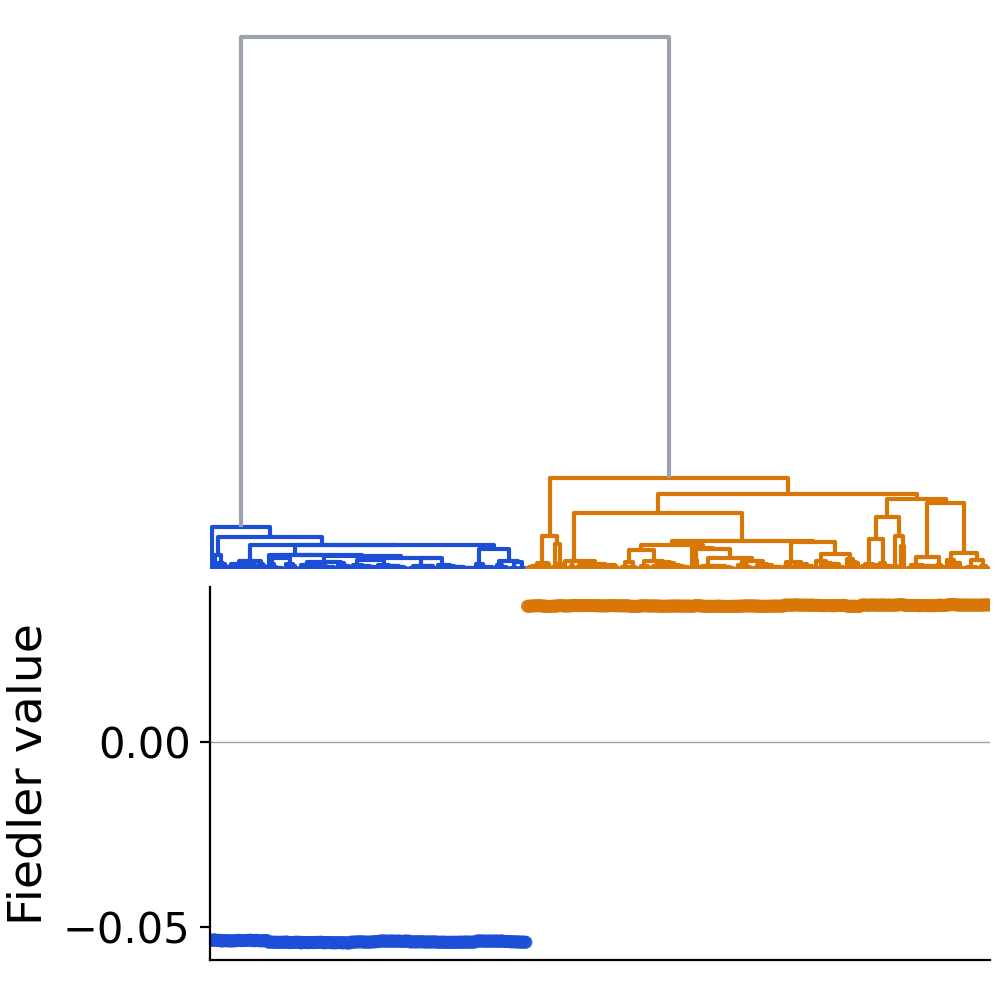
\includegraphics[width=\textwidth]{Fiedler_Bipartitions/fiedler_tree_partition_eta01.png}
\end{subfigure}
\hfill{\color{black!25}\rule[-5.0cm]{0.4pt}{5.0cm}}\hfill
\begin{subfigure}[t]{0.30\textwidth}
  \captionsetup{singlelinecheck=false, justification=raggedright, skip=1pt}
  \subcaption{$\eta=4.4$}\label{fig:fied-eta05}
  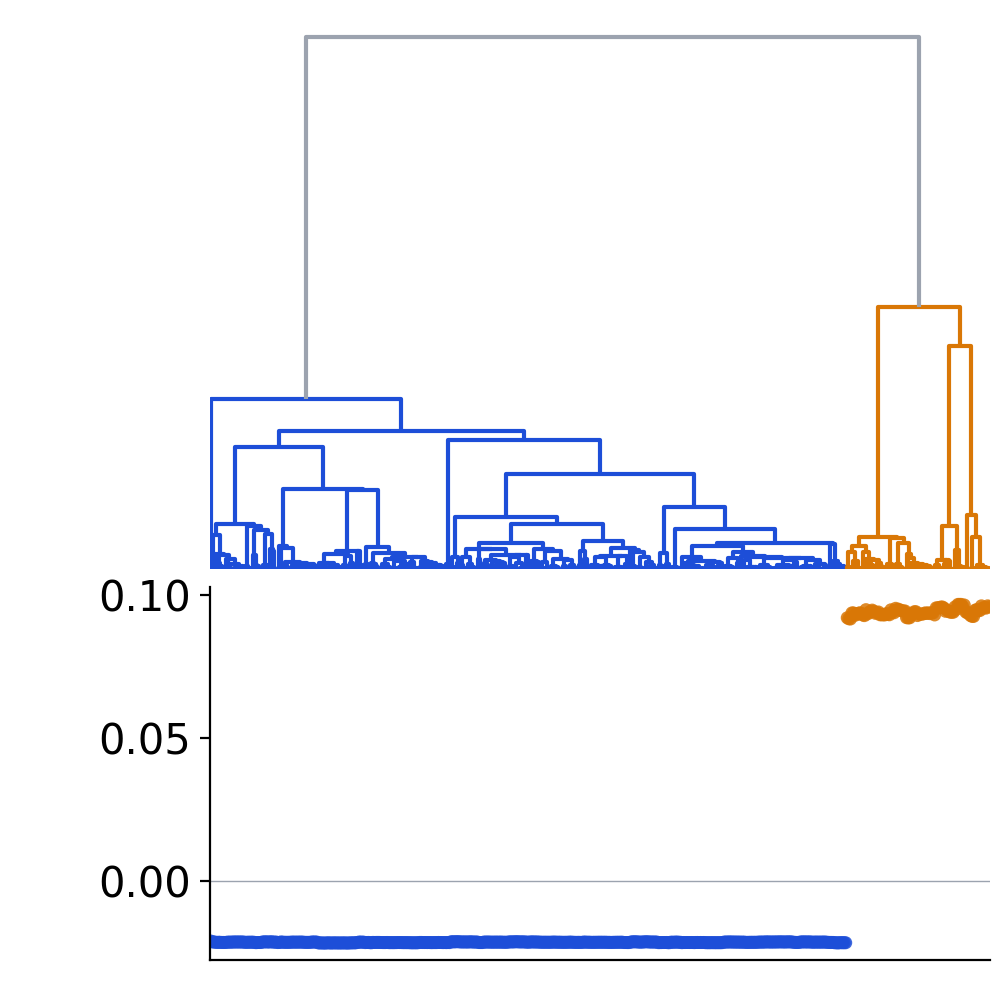
\includegraphics[width=\textwidth]{Fiedler_Bipartitions/fiedler_tree_partition_eta05.png}
\end{subfigure}
\hfill{\color{black!25}\rule[-5.0cm]{0.4pt}{5.0cm}}\hfill
\begin{subfigure}[t]{0.30\textwidth}
  \captionsetup{singlelinecheck=false, justification=raggedright, skip=1pt}
  \subcaption{$\eta=15.1$}\label{fig:fied-eta15}
  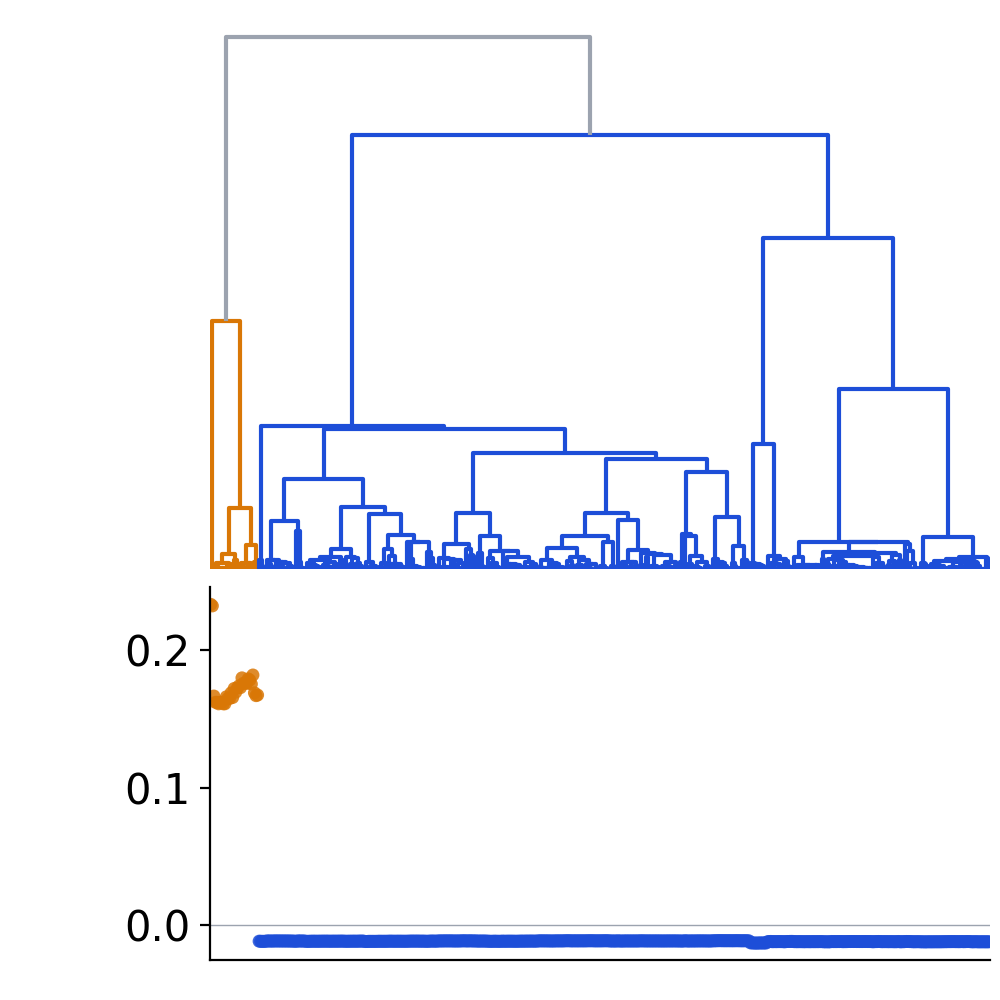
\includegraphics[width=\textwidth]{Fiedler_Bipartitions/fiedler_tree_partition_eta15.png}
\end{subfigure}
\caption{$\Pisp{S}$ on three trees, one per panel. Each is drawn
from a pool of simulated Kingman trees ($m=500$ terminal nodes, JC69 sequences of length
$\ell=10^4$) binned by the imbalance its Fiedler split realises. In each panel the
tree is on top, its branches coloured by the sign of the Fiedler vector --- grey on
the one branch that spans both signs --- and below it the Fiedler value of each terminal node
is plotted at that node's own horizontal position in the tree. The sign pattern cuts a single edge
every time, as \Cref{thm:stdr-split} requires, and the smaller the clade it cuts off, the
larger the values carried by its terminal nodes.}
\label{fig:fiedler_partitions}
\end{figure}
         % §4  Modelling assumptions            (sec:assumptions)
% §4 Main result.  Delivers one theorem: p = Theta(log m / m) suffices for the entry-wise
% criterion eq:entrywise to hold w.h.p.  The statement is about the criterion, not about
% which split of the tree is returned -- that is §5.
\section{Main Result}\label{sec:main}
The entry-wise recovery criterion \eqref{eq:entrywise} is what the sampling rate
has to buy. This section converts it into a sufficient condition on $p$ for the
Laplacian $L=D-S$, stated in the structural quantities of \Cref{sec:assumptions}: the
margin $\rho$ of \eqref{eq:margin_definition} and the imbalance $\eta$ of
\eqref{eq:imbalance_ratio}.

\begin{theorem}[Exact recovery of the full-data split]\label{thm:main-sim}
Let $S$ satisfy the constant block model of \Cref{def:cfbm} with $m$ terminal nodes and
imbalance $\eta\ge1$, let $\rho$
be the structural margin and let $\vvh$ be the empirical Fiedler vector --- the
unit eigenvector belonging to the second-smallest eigenvalue of the sampled
Laplacian $\hat L=\hat D-\hat S$, formed from entries observed with probability
$p$ as in the observation model \eqref{eq:sampling_estimator}. Assume
\Cref{asm:margin}. For the entry-wise recovery criterion
\eqref{eq:entrywise} to hold \hp, i.e.\
$\norm{\vvh-\vv}_\infty<\min_i|\vv_i|$, it suffices that
\begin{equation}\label{eq:main_rate}
   p\;>\;\frac{8(1+\eta)^3\,\bze^2\,\log m}{m\,(\rho-\eta\,\bze)^2}
       \;=\;\Theta\!\left(\frac{\log m}{m}\right).
\end{equation}
\end{theorem}

\noindent \eqref{eq:main_rate} is a \emph{sufficient} condition. No matching lower
bound is proved anywhere in this paper, so the $\Theta(\log m/m)$ is the growth
order of that sufficient bound and not a claim that the rate is tight or
order-optimal.

         % §5  Main Result                      (sec:main)
% §5 Topological scaling and spectral gap.  No sampling enters.  Exact statements about
% the population Laplacian, delivering which split Pi(S) is and how eta moves the
% coherence and the gap until recovery becomes impossible.
% §6 consumes lem:A-decomp and lem:gap from here.
\section{Topological Scaling and Spectral Gap}\label{sec:bridging}

This section deals with how the macro-topology of $\mathcal{T}$ fixes its spectrum: the eigenpair that carries the
split it carries, the coherence of the leading invariant subspace, and the gap
separating $\lambda_2$ from $\lambda_3$. The whole dependence runs through the single
structural parameter $\eta$ of \Cref{def:imbalance}.

\begin{lemma}[Spectral decomposition of the imbalanced Laplacian]\label{lem:A-decomp}
Let $S$ satisfy \Cref{def:cfbm} at a bipartition $\mathcal{X}=C_1\cup C_2$, as \Cref{prop:cfbm}
guarantees at the root split
under \Cref{asm:gtr,asm:clock}. Then (i) the smallest eigenvalue of $L$ is
$\lambda_1=0$, simple, with $v^{(1)}=\tfrac1{\sqrt m}\1_m$; (ii) $m\bze$ is an
eigenvalue of $L$ whose eigenvector is piecewise constant on the split,
$\vv_i=+c_1$ for $i\in C_1$ and $\vv_i=-c_2$ for $i\in C_2$, with $c_1=\sqrt{|C_2|/(|C_1|m)}$
and $c_2=\sqrt{|C_1|/(|C_2|m)}$; and (iii) consequently
\begin{equation}\label{eq:lambda2_upper}
   \lambda_2 \le m\bze .
\end{equation}
If in addition \Cref{asm:margin} holds, then (iv) \eqref{eq:lambda2_upper} holds with
equality: $\lambda_2=m\bze$ is simple and $\vv$ is the Fiedler vector of the
similarity graph.
\end{lemma}

\noindent The proof is in \Cref{app:comp1}. Clauses (i)--(iii) are a direct
computation, and they use only the constancy of the cross-block, not the floor:
the identity $(D_{C_1}-S_{C_1})\1_{|C_1|}=|C_2|\bze\1_{|C_1|}$ holds for an arbitrary symmetric diagonal
block, because $D_{C_1}$ already carries the row sums of that block. Clause (iv) is where
\Cref{asm:margin} enters, as the statement that $m_{\min}\Sin^{\min}>m\bze$: it puts
the interlacing lower bound on $\lambda_3$ used in \Cref{lem:gap} strictly above
$m\bze$, leaving no eigenvalue between $0$ and $m\bze$. It is what makes
$\min_i|\vv_i|=c_2$ available to the proof of \Cref{thm:main-sim}. Since $\vv$ is
non-negative exactly on $C_1$, the sign rule \eqref{eq:sign_rule} returns $C_1$ as its
first block, so the labelling of \Cref{def:imbalance} and that of \Cref{thm:stdr-split}
agree: $C_1$ is the smaller clade.

\subsection{Coherence and the spectral gap under imbalance}\label{sec:bridging-scaling}

Two scalar quantities of the population Laplacian sit behind the constants of
\eqref{eq:main_rate}, and $\eta$ moves both against recovery. The first is the
spectral gap that isolates the Fiedler vector,
\begin{equation}\label{eq:gap_definition}
   \Dlam := \lambda_3 - \lambda_2 ,
\end{equation}
with $\lambda_2,\lambda_3$ as in \Cref{def:fiedler}. The second measures how evenly
the leading invariant subspace of $L$ spreads across nodes.

\begin{definition}[Subspace coherence]\label{def:coherence}
Let $U=[v^{(1)},\vv]\in\R^{m\times2}$ span the invariant subspace of the two
smallest eigenvalues of $L$, with $v^{(1)}=\tfrac1{\sqrt m}\1_m$ the trivial flat
eigenvector and $\vv$ the Fiedler vector. The \emph{subspace coherence} is
\begin{equation}\label{eq:coherence_definition}
   \coh := \tfrac{m}{2}\max_{1\le i\le m}\norm{P_U e_i}_2^2
         = \tfrac{m}{2}\max_{1\le i\le m}\bigl((v_i^{(1)})^2+(\vv_i)^2\bigr),
   \qquad P_U=UU^\top.
\end{equation}
\end{definition}

\noindent Coherence is minimal, $\coh=1$, when the subspace is spread evenly, and
grows as it localizes onto few coordinates. Both quantities are fixed by
 macro-topological features alone: $\eta$ first inflates $\coh$, then erodes $\Dlam$.

\begin{proposition}[Topological scaling of coherence]\label{prop:coherence}
Under \Cref{def:cfbm}, the tree imbalance $\eta$ maps deterministically to the
subspace coherence,
\begin{equation}\label{eq:coherence_linear_growth}
   \coh=\frac{1+\eta}{2}.
\end{equation}
\end{proposition}
\noindent The identity follows by substituting the Fiedler coordinates of
\Cref{lem:A-decomp} into \eqref{eq:coherence_definition}; the short computation is given in
\Cref{app:comp1}. Thus a balanced split attains the
optimal coherence $\coh=1$, and the signal spreads more unevenly across nodes as
$\eta$ grows; the generated regime of \Cref{sec:empirical} confirms the identity
on data from the full generative pipeline. The identity is reported as a
structural diagnostic: since the noise bound of \Cref{lem:B-bernstein} is obtained
from the row norms of $S$ directly (\Cref{app:comp2}), $\coh$ does not itself enter
the sampling rate, and the $\eta$-dependence of \eqref{eq:main_rate} arrives
through the margin and the gap instead.


The gap $\Dlam$ of \eqref{eq:gap_definition} is the quantity the perturbation
argument of \Cref{sec:outline} divides by, and the same imbalance that raises $\coh$
drives it toward zero.

\begin{lemma}[Spectral-gap lower bound]\label{lem:gap}
Let $L$ be the combinatorial Laplacian of a similarity matrix satisfying the
molecular clock, with structural margin $\rho$ as in \eqref{eq:margin_definition}. For
$m_{\min}=\min(|C_1|,|C_2|)$ and imbalance $\eta$, the spectral gap isolating the Fiedler
vector satisfies
\begin{equation}\label{eq:spectral_gap_margin}
   \Dlam \ge m_{\min}\rho-\eta\,m_{\min}\,\bze.
\end{equation}
\end{lemma}
\noindent The full algebraic-connectivity derivation is given in \Cref{app:comp1},
building on the eigenpairs of \Cref{lem:A-decomp}. The bound
\eqref{eq:spectral_gap_margin} is purely a CBM statement, controlling the gap
through the abstract minimum within-block similarity $\Sin^{\min}$ of
\eqref{eq:cfbm_floor}.

\subsection{Two failure modes}\label{sec:bridging-failure}

\Cref{prop:coherence} and \Cref{lem:gap} show that the same parameter $\eta$ acts
on both spectral quantities at once, which produces two distinct ways for
top-down recovery to fail; together they bound the admissible region of
$(m,\eta)$. The first is \emph{structural collapse},
$\Dlam\to0$, which we state here as a corollary of the gap lemma; the second is
\emph{statistical infeasibility}, $p>1$, which is a consequence of
\Cref{thm:main-sim}. A positive gap requires the structural margin to
dominate the imbalance-weighted cross-block boundary,
$m_{\min}\rho>\eta\,m_{\min}\bze$, i.e.\
$\eta<\Sin^{\min}/\bze$ --- precisely what \Cref{asm:margin} records.
Translating this
ratio into tree distances bounds the imbalance the topology can sustain.

\begin{corollary}[Structural imbalance tolerance]\label{cor:tolerance}
Measure the tree in log-similarity units: by \eqref{eq:similarity_gtr},
$r(\mathcal T):=\max_{i,j}(-\log S_{ij})=|\mathrm{tr}(Q)|\max_{i,j}d_{ij}$ is its diameter,
and $h(\mathcal T)$ its depth in the same units \cite{aizenbud2023spectral}, with
$h(\mathcal T)<r(\mathcal T)$.
Then a positive spectral gap is possible only if
\begin{equation}\label{eq:eta_distance_bound}
   \eta\le\mathcal O\!\bigl(e^{\mathcal O(h(\mathcal T))-r(\mathcal T)}\bigr).
\end{equation}
In particular, for an average Kingman coalescent tree, where
$r(\mathcal T),h(\mathcal T)=\mathcal O(\log m)$
\cite{erdos1999logs, aldous2001stochastic}, this gives $\eta\le\mathcal O(m^c)$ for
a model-dependent constant $c$.
\end{corollary}
\noindent The proof sketch (substituting the diameter/depth bounds into
$\eta<\Sin^{\min}/\bze$) is given in \Cref{app:comp1}.

So under balanced generative models the gap survives polynomial imbalance. A
positive gap is necessary but not sufficient: even when $\Dlam>0$, the rate
\eqref{eq:main_rate} grows with $\eta$, and the second failure mode is the imbalance
past which that demand exceeds $p=1$.

\begin{corollary}[Vacuity of the certificate under imbalance]\label{cor:infeasible}
Under the hypotheses of \Cref{thm:main-sim}, with $\bze$ and the margin
$\rho-\eta\bze$ held bounded away from $0$ independently of $\eta$, the
right-hand side of \eqref{eq:main_rate} exceeds $1$ once
$\eta=\Omega\!\bigl(\sqrt[3]{m/\log m}\bigr)$; in general the threshold is
reached when $\eta^3\bze^2/(\rho-\eta\bze)^2=\Omega(m/\log m)$. No admissible sampling rate
$p\in(0,1]$ then satisfies the sufficient condition, so \Cref{thm:main-sim}
certifies nothing in that regime. What the theorem stops certifying there is the
sampling: \Cref{thm:stdr-split} continues to make $\Pisp{S}$ a split of
$\mathcal{T}$ whatever $\eta$ does.
\end{corollary}
 % §6  Topological scaling, spectral gap (sec:bridging)
% §6 Proof outline.  Delivers the three stages that turn eq:entrywise into eq:main_rate:
% matrix-Bernstein noise bound, Neumann entry-wise reduction, per-node concentration.
% Proofs themselves are in the appendices.
\section{Proof Outline}\label{sec:outline}
The proof of \Cref{thm:main-sim} compares two quantities evaluated at the same
node: the entry-wise error $|\vvh_i-\vv_i|$ and the entry-wise margin $|\vv_i|$.
It runs in three stages --- population geometry fixes the margin and noise
budget, a resolvent expansion reduces the error at each node to a scalar, and a
per-node Bernstein bound controls that scalar --- after which imposing
\eqref{eq:entrywise} yields the rate \eqref{eq:main_rate}. Each stage is stated
as a lemma; the proofs are in \Cref{app:comp1,app:comp2,app:comp3}.

\emph{Stage 1 (population geometry and noise budget).} The same imbalance $\eta$
sets both sides of \eqref{eq:entrywise} at once --- it fixes the margin and the
spectral gap through the piecewise-constant Fiedler vector of
\Cref{lem:A-decomp} and the gap bound of \Cref{lem:gap}, kept positive by
\Cref{asm:margin}, while on the other side matrix Bernstein applied to the
sampling mask bounds the noise the gap has to absorb.

\begin{lemma}[Laplacian spectral error via matrix Bernstein]\label{lem:B-bernstein}
Under \Cref{def:cfbm} and the observation model
\eqref{eq:sampling_estimator}, there are constants $\tilde C,C_0$
such that if $p\ge C_0\,\tfrac{\log m}{m}$ then \hp
\[
   \opnorm{\EL}\le\tilde C\sqrt{\frac{m\log m}{p}}.
\]
\end{lemma}
\noindent The proof is in \Cref{app:comp2}. Compared against the gap bound of
\Cref{lem:gap}, this is what certifies the strong-signal regime
$\opnorm{\EL}<\Dlam$ that the next stage assumes. Under imbalance the margin and
the gap are extremal at different nodes, which is what makes the final synthesis
$\eta$-dependent.

\emph{Stage 2 (entry-wise reduction).} Since \eqref{eq:entrywise} is an
$\ell_\infty$ event while Davis--Kahan controls only $\ell_2$, and the sole
dimension-free transfer between them, $\norm{\cdot}_\infty\le\norm{\cdot}_2$,
charges every node as though it were the worst one, the reduction has to be
coordinate-wise: in the regime of Stage 1 a resolvent (Neumann) expansion of
$\vvh$ in $\EL$ trades the operator norm for a single scalar per coordinate, at
the price of a remainder that is second order in the noise-to-gap ratio.

\begin{lemma}[Neumann decomposition of the Fiedler vector]\label{lem:neumann}
Let $L$ be symmetric with eigenpairs $\{(\lambda_\ell,v^{(\ell)})\}$, let
$\hat L=L+\EL$ be a symmetric perturbation, and write $\vvh=\vv+w$. If
$\opnorm{\EL}<\Dlam$, then, with $\Pi$ the spectral projector onto the complement
of $\vv$, $w$ admits the exact resolvent expansion
$w=\sum_{k\ge1}(-1)^k(\Dlam^{-1}\Pi\EL)^k\vv$, whose first-order term is
\begin{equation}\label{eq:neumann_first_order}
   w^{(1)}=\sum_{\ell\ne2}\frac{-\langle v^{(\ell)},\EL\vv\rangle}
        {\lambda_\ell-\hat\lambda_2}\,v^{(\ell)},
\end{equation}
so that entrywise $w_i=-(\EL\vv)_i/\Dlam+R_i$ with the remainder of second order,
$\norm{R}_\infty=O\!\bigl(\opnorm{\EL}^2/\Dlam^2\bigr)$.
\end{lemma}
\noindent The expansion is due to Eldridge et al.\
\cite{eldridge2017unperturbed}, Fan et al.\ \cite{fan2018eigenvector} and Abbe
et al.\ \cite{abbe2020entrywise} rather than to this paper, which is why it is
stated as a lemma; the decomposition and its first-order bound are proved in
\Cref{app:comp3a}, and the remainder $R$ separately in \Cref{app:comp3c}
(\Cref{lem:C-remainder}), its discard being what confines the argument to the
strong-signal regime of Stage 1.

\emph{Stage 3 (per-node concentration).} The surviving scalar $(\EL\vv)_i$ is a
sum of independent, mean-zero increments, each carrying the factor $\vv_i-\vv_j$.
Every within-block increment therefore vanishes \emph{exactly} --- this is a
cancellation, not a bound, and it rests on the clock (\Cref{asm:clock}) making
$\vv$ exactly piecewise constant, so it is the one step that would degrade if the
cross-block were only approximately constant. Only cross-block pairs survive,
Bernstein's inequality applies node by node, and since this is the only place the
sampling rate $p$ enters the final condition, we state the bound in the main text.

\begin{lemma}[Per-node concentration]\label{lem:pernode}
With scale $R_2=\bze(1+\eta)/(p\sqrt{m\eta})$, for each $i\in C_2$ and $\delta>0$,
with probability $\ge1-\delta$,
$|(\EL\vv)_i|\le2\sqrt{2\sigma_2^2\ln(2/\delta)}+\tfrac23R_2\ln(2/\delta)$. In the
variance-dominated regime ($p=\Theta(\log m/m)$), a union bound over all $m$ nodes
at $\delta=\delta_0/m$ gives, \hp\ uniformly over $i$,
\begin{equation}\label{eq:concentration-bound}
   |(\EL\vv)_i|\lesssim\sqrt{\frac{8(1+\eta)\bze^2\log(2m/\delta_0)}{\eta\,p}}.
\end{equation}
\end{lemma}
\noindent The increment representation, the cancellation of the within-block
pairs, the per-node variance $\sigma_2^2$ and the proof are in
\Cref{app:comp3b}. This is the step that realises the $\sqrt m$ saving that the
Davis--Kahan route forfeits: the variance of the increment sum is smaller than
$\opnorm{\EL}^2$ by a factor $m$, and it is this per-coordinate saving that turns
\eqref{eq:entrywise} into the rate \eqref{eq:main_rate}; \Cref{app:compare} runs
the two routes side by side and \Cref{rem:E-compare} reports the ratio. The three
stages now combine.

\begin{proof}[Proof of \Cref{thm:main-sim}]
\emph{Step 1 (population geometry).} \Cref{lem:A-decomp,lem:gap} supply the
right-hand side of \eqref{eq:entrywise} as $\min_i|\vv_i|=c_2$ and a spectral gap
$\Dlam$ that is positive under \Cref{asm:margin}, and \Cref{lem:B-bernstein}
places $\opnorm{\EL}$ below it.

\emph{Step 2 (entry-wise reduction).} \Cref{lem:neumann} is therefore applicable
and gives $w_i=-(\EL\vv)_i/\Dlam+R_i$; discarding $R$ as lower order against
$c_2$ reduces \eqref{eq:entrywise} to the per-node condition
$|(\EL\vv)_i|<\Dlam|\vv_i|$ holding at every node $i$.

\emph{Step 3 (concentration).} \Cref{lem:pernode} bounds the left-hand side of
that condition uniformly over the $m$ nodes.

\emph{Step 4 (synthesis).} The per-node condition is tightest on clade $C_2$, since
$\eta\ge1$. Squaring $\sqrt{8\sigma_2^2\log m}<\Dlam c_2$ and substituting
$\sigma_2^2$, $c_2^2=1/(m\eta)$ and the gap bound
$\Dlam\ge m_{\min}(\rho-\eta\bze)$, the factor $\eta$ cancels and solving
for $p$ gives exactly \eqref{eq:main_rate}
(\Cref{prop:C-bind} and \Cref{cor:C-cond}). Under \eqref{eq:main_rate} every node satisfies
$|w_i|<|\vv_i|$, hence $\vvh_i$ and $\vv_i$ share a sign; since $\vv$ is
sign-constant on each clade (\Cref{lem:A-decomp}), the zero-threshold partition of
$\vvh$ is $(C_1,C_2)$ exactly.
\end{proof}

       % §7  Proof outline                    (sec:outline)
% §7 Empirical study.  Point: measure the price of sampling -- the agreement between the
% sub-sampled and the full-data partition -- on closed-form and on simulated matrices,
% for both operators.  It does not certify which split of a tree either partition is.
\section{Empirical Results}\label{sec:empirical}

Two experiments produce the figures below. In the first, $S$ is written down directly from the constant block model of \Cref{def:cfbm} with $\Sin^{\min}=0.9$ and $\bze=0.05$, so the sampling mask is the only source of error. In the second, dendropy simulates Kingman coalescent trees, evolves JC69 sequences of length $\ell=10^4$ along their branches, and $S$ is the log-det similarity estimated from the resulting alignment (\Cref{asm:gtr}); tree shape is then off-model and every entry of $S$ carries estimation noise, so this is where the exact cross-block baseline of \Cref{asm:clock} and the margin of \Cref{asm:margin} are put to the test.

Each matrix is sub-sampled independently at every $p$ on a grid and read through the Laplacian $L$ of \Cref{thm:main-sim}, rounded by $k$-means on $L_{\mathrm{sym}}$ as that theorem prescribes. A point is an average over $20$ independent sub-sampling replicates at that size and imbalance; on the simulated trees the count is set by how many trees the pool holds at that $(n,\eta)$.

Recovery is scored by the Normalized Mutual Information (NMI) between the split $\Pisp{\hat S}$ returned from the sub-sampled matrix and the reference split $\Pisp{S}$ returned by the same operator on the full matrix at $p=1$. NMI is the standard measure of agreement between two spectral-clustering partitions \cite{fortunato2010community, qinrohe2013regularized}:
\begin{equation}\label{eq:nmi_def}
   \mathrm{NMI}(Y,C)=\frac{2\,I(Y;C)}{H(Y)+H(C)},
\end{equation}
with $I(Y;C)$ the mutual information and $H(\cdot)$ the Shannon entropy. NMI attains its maximum value $1$ if and only if the two partitions are identical up to relabeling, and decays as they disagree \cite{strehlghosh2002cluster, fortunato2010community}. The quantity being measured is therefore the cost of sub-sampling and nothing else: both partitions come from the same operator on the same tree, and they differ only in how many entries of $S$ were computed.

\begin{corollary}[Perfect partition recovery and $\mathrm{NMI}=1$]\label{cor:nmi}
Under the hypotheses of \Cref{thm:main-sim}, the partition $\Pisp{\hat S}$ obtained by thresholding $\vvh$ at zero satisfies $\Pisp{\hat S}=\Pisp{S}$ \hp, and therefore $\mathrm{NMI}(\Pisp{\hat S},\Pisp{S})=1$.
\end{corollary}
\begin{proof}
\Cref{thm:main-sim} guarantees $\norm{\vvh-\vv}_\infty<\min_i|\vv_i|$, so for each node $i$, $|\vvh_i-\vv_i|<|\vv_i|$, which forces $\vvh_i$ and $\vv_i$ to share a sign. Thresholding both at zero therefore yields the same partition, $\Pisp{\hat S}=\Pisp{S}$. No property of the tree enters: the argument is node-wise sign agreement between two vectors. Exact agreement gives $I(\Pisp{\hat S};\Pisp{S})=H(\Pisp{\hat S})=H(\Pisp{S})$, whence by \eqref{eq:nmi_def} $\mathrm{NMI}(\Pisp{\hat S},\Pisp{S})=1$.
\end{proof}

Both figures below share one layout: one pair of panels per imbalance, at $\eta=1,5,10,15$ throughout. On the left, measured NMI against the sampling rate $p$, one curve per size, the curves running dark to light (viridis) with increasing size, and the red dashed line at the $0.90$ level that defines the empirical threshold $\hat p^\star$. On the right, $\hat p^\star$ against size on log-log axes, with a dotted reference of the shape \eqref{eq:main_rate} predicts, $\log m/m$, fitted to the measured points. Filled markers are measured; open markers are bounds rather than thresholds, a read-off pinned at either end of the $p$ grid, and are excluded from the fit.

Along the similarity route the transition sharpens and shifts left as the size grows, and $\hat p^\star$ decays parallel to the reference at every $\eta$ on both data sets: on the closed-form matrix of \Cref{fig:pstar_synth}, and on the simulated phylogenies of \Cref{fig:pstar_gen}, where the coherence and gap identities of \Cref{prop:coherence} and \Cref{lem:gap} continue to hold despite off-model tree shapes and JC69 noise. The $\Theta(\log m/m)$ sample complexity of \eqref{eq:main_rate} therefore survives finite-sequence estimation noise.

\begin{figure}[t]
    \centering
    \begin{subfigure}[t]{0.49\textwidth}
        \captionsetup{singlelinecheck=false, justification=raggedright, skip=1pt}
        \subcaption{$\eta=1$}\label{fig:pstar_synth_eta1}
        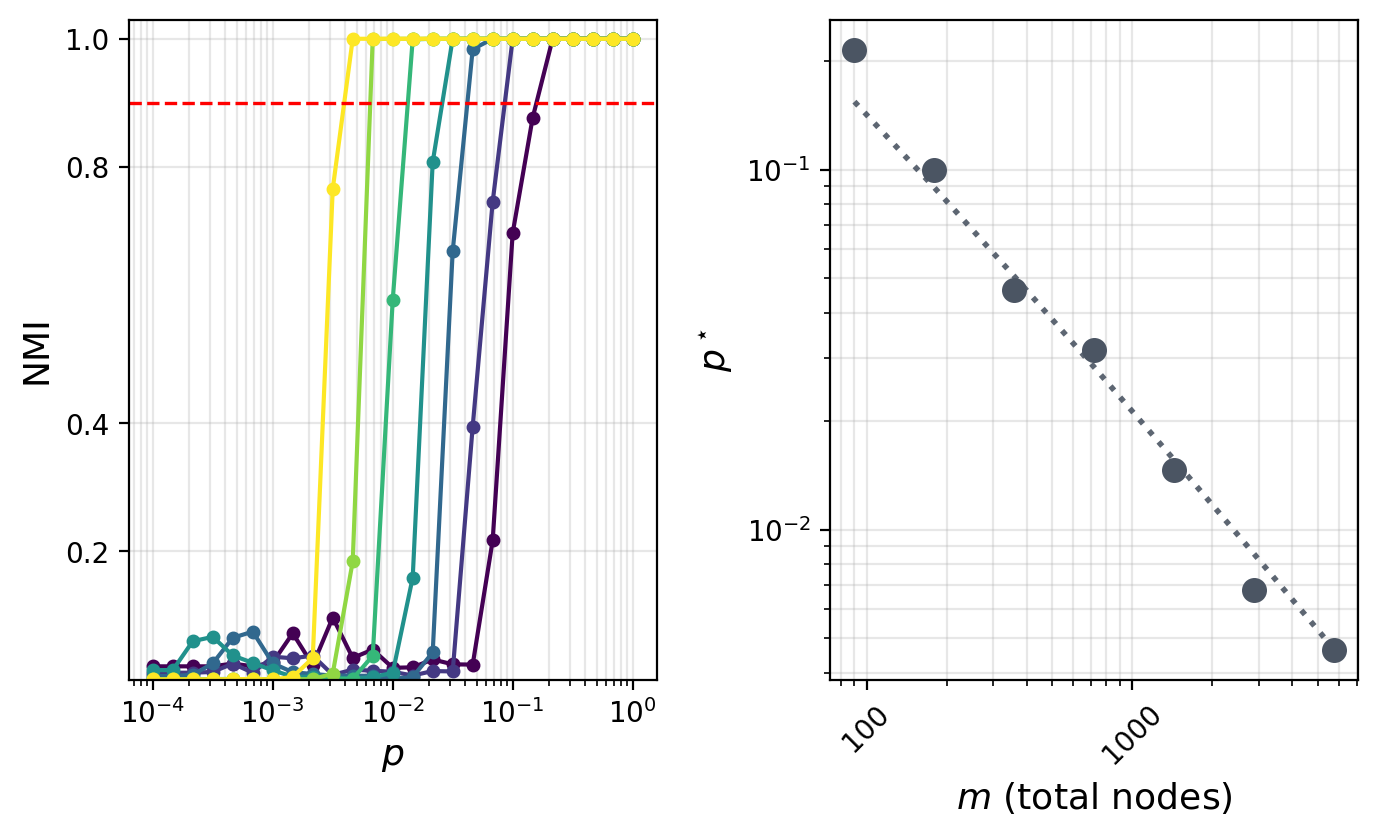
\includegraphics[width=\textwidth]{pstar_synth_nmi_eta1.png}
    \end{subfigure}
    \hfill
    \begin{subfigure}[t]{0.49\textwidth}
        \captionsetup{singlelinecheck=false, justification=raggedright, skip=1pt}
        \subcaption{$\eta=5$}\label{fig:pstar_synth_eta5}
        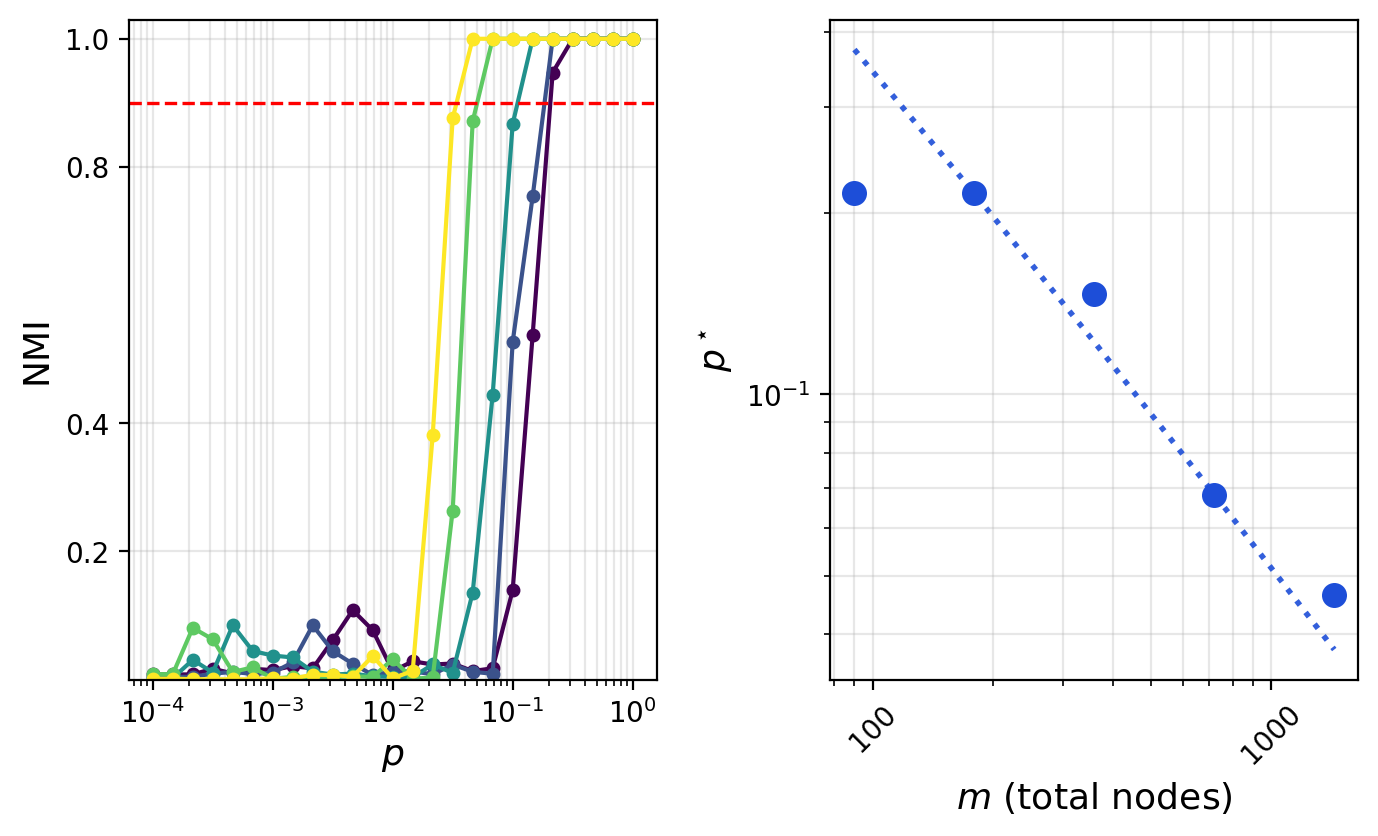
\includegraphics[width=\textwidth]{pstar_synth_nmi_eta5.png}
    \end{subfigure}

    \vspace{3mm}

    \begin{subfigure}[t]{0.49\textwidth}
        \captionsetup{singlelinecheck=false, justification=raggedright, skip=1pt}
        \subcaption{$\eta=10$}\label{fig:pstar_synth_eta10}
        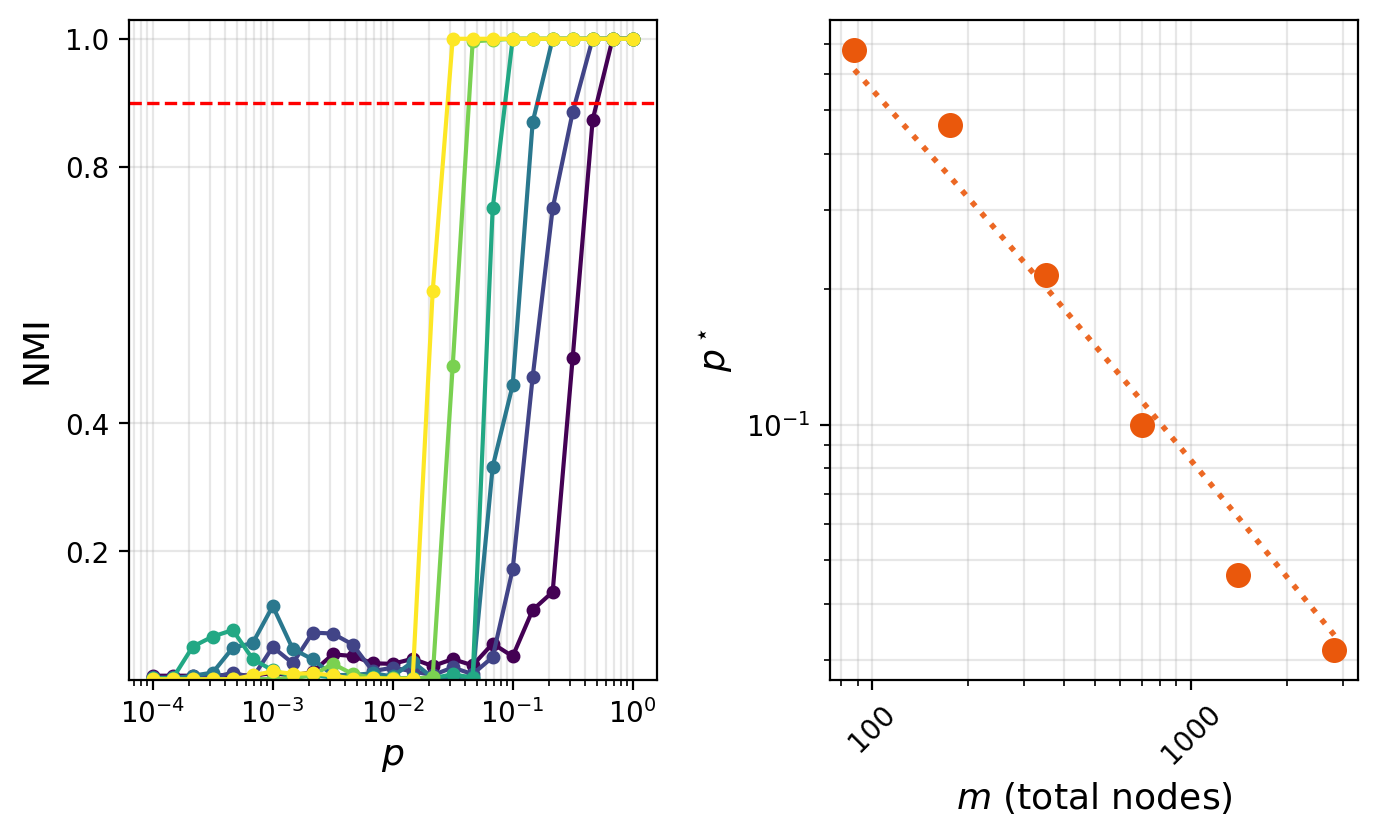
\includegraphics[width=\textwidth]{pstar_synth_nmi_eta10.png}
    \end{subfigure}
    \hfill
    \begin{subfigure}[t]{0.49\textwidth}
        \captionsetup{singlelinecheck=false, justification=raggedright, skip=1pt}
        \subcaption{$\eta=15$}\label{fig:pstar_synth_eta15}
        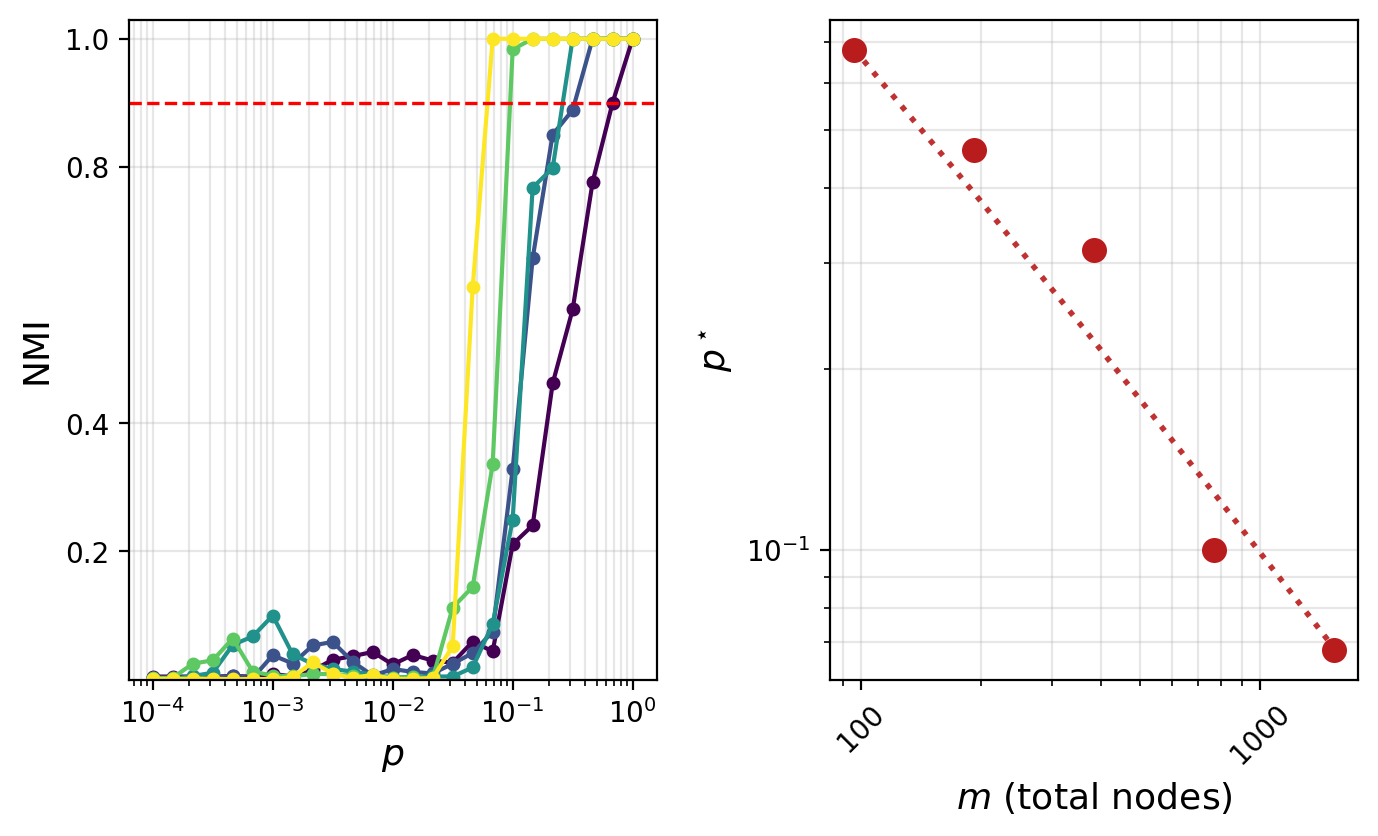
\includegraphics[width=\textwidth]{pstar_synth_nmi_eta15.png}
    \end{subfigure}
    \caption{\textbf{Similarity route, no estimation noise.} $S$ is the constant block model
    of \Cref{def:cfbm} in closed form, so the sampling mask is the only error present. The
    transition sharpens and moves left as $m$ grows, and $\hat p^\star$ falls parallel
    to $\log m/m$ at every imbalance.}
    \label{fig:pstar_synth}
\end{figure}

\begin{figure}[t]
    \centering
    \begin{subfigure}[t]{0.49\textwidth}
        \captionsetup{singlelinecheck=false, justification=raggedright, skip=1pt}
        \subcaption{$\eta\approx1$}\label{fig:pstar_gen_eta1}
        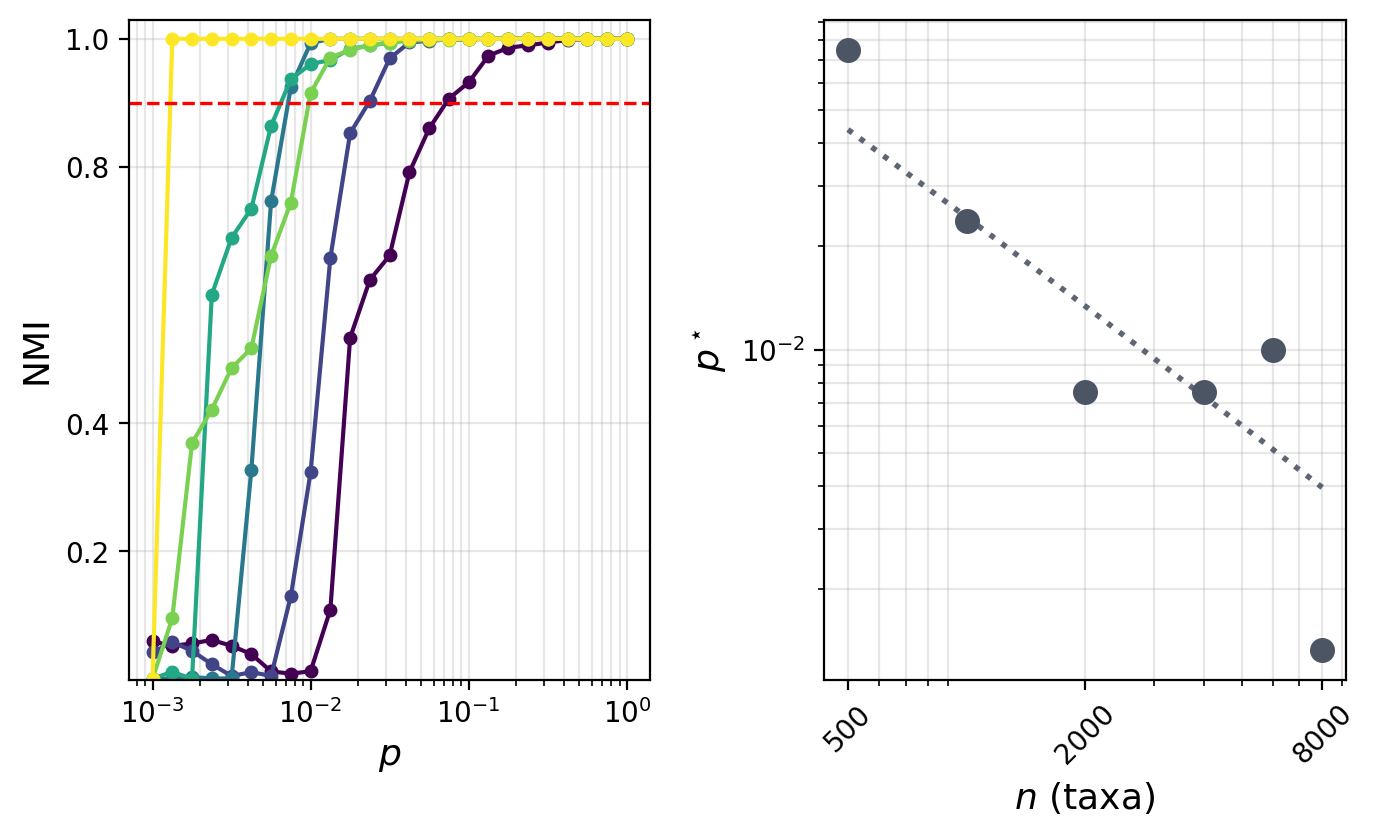
\includegraphics[width=\textwidth]{pstar_gen_kmeans_eta1.png}
    \end{subfigure}
    \hfill
    \begin{subfigure}[t]{0.49\textwidth}
        \captionsetup{singlelinecheck=false, justification=raggedright, skip=1pt}
        \subcaption{$\eta\approx5$}\label{fig:pstar_gen_eta5}
        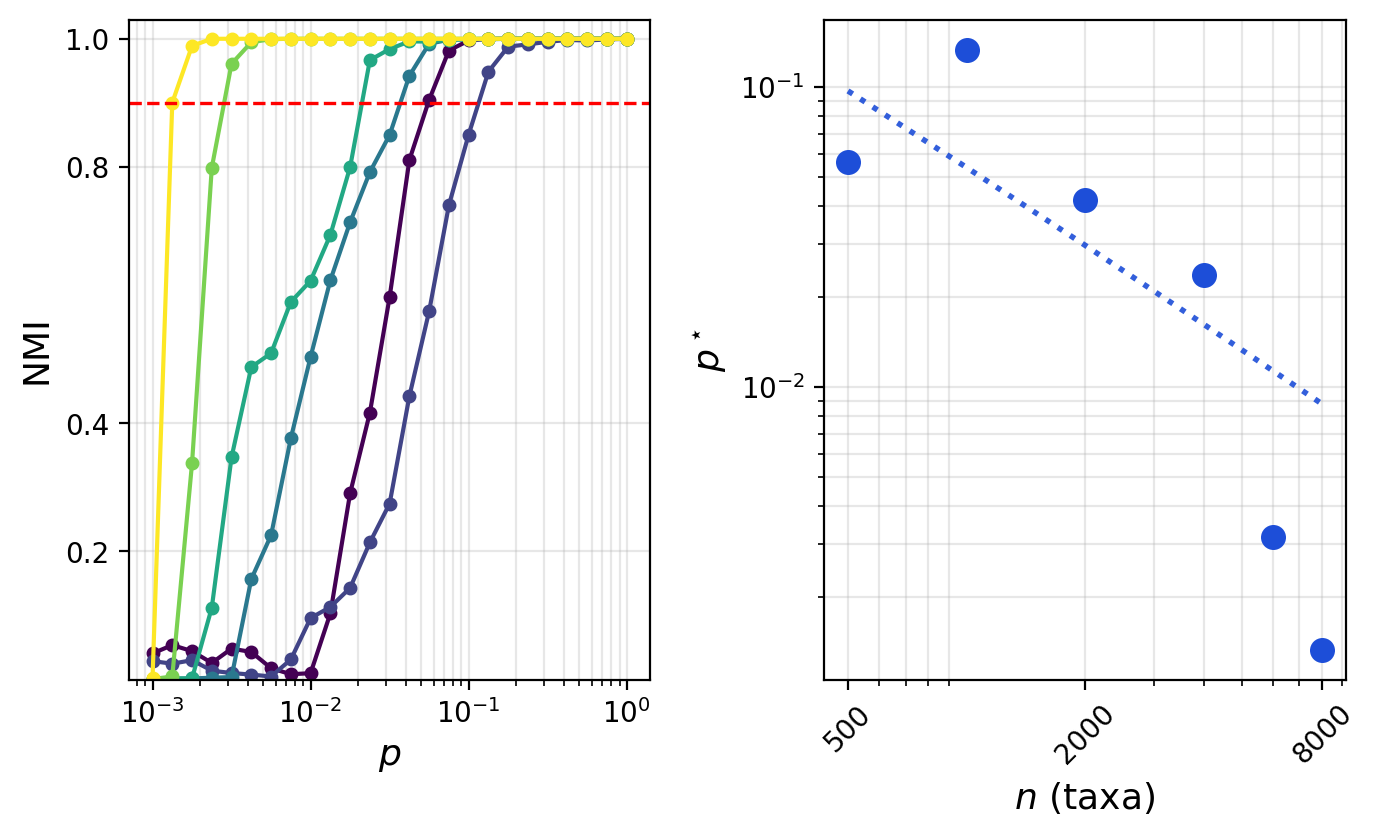
\includegraphics[width=\textwidth]{pstar_gen_kmeans_eta5.png}
    \end{subfigure}

    \vspace{3mm}

    \begin{subfigure}[t]{0.49\textwidth}
        \captionsetup{singlelinecheck=false, justification=raggedright, skip=1pt}
        \subcaption{$\eta\approx10$}\label{fig:pstar_gen_eta10}
        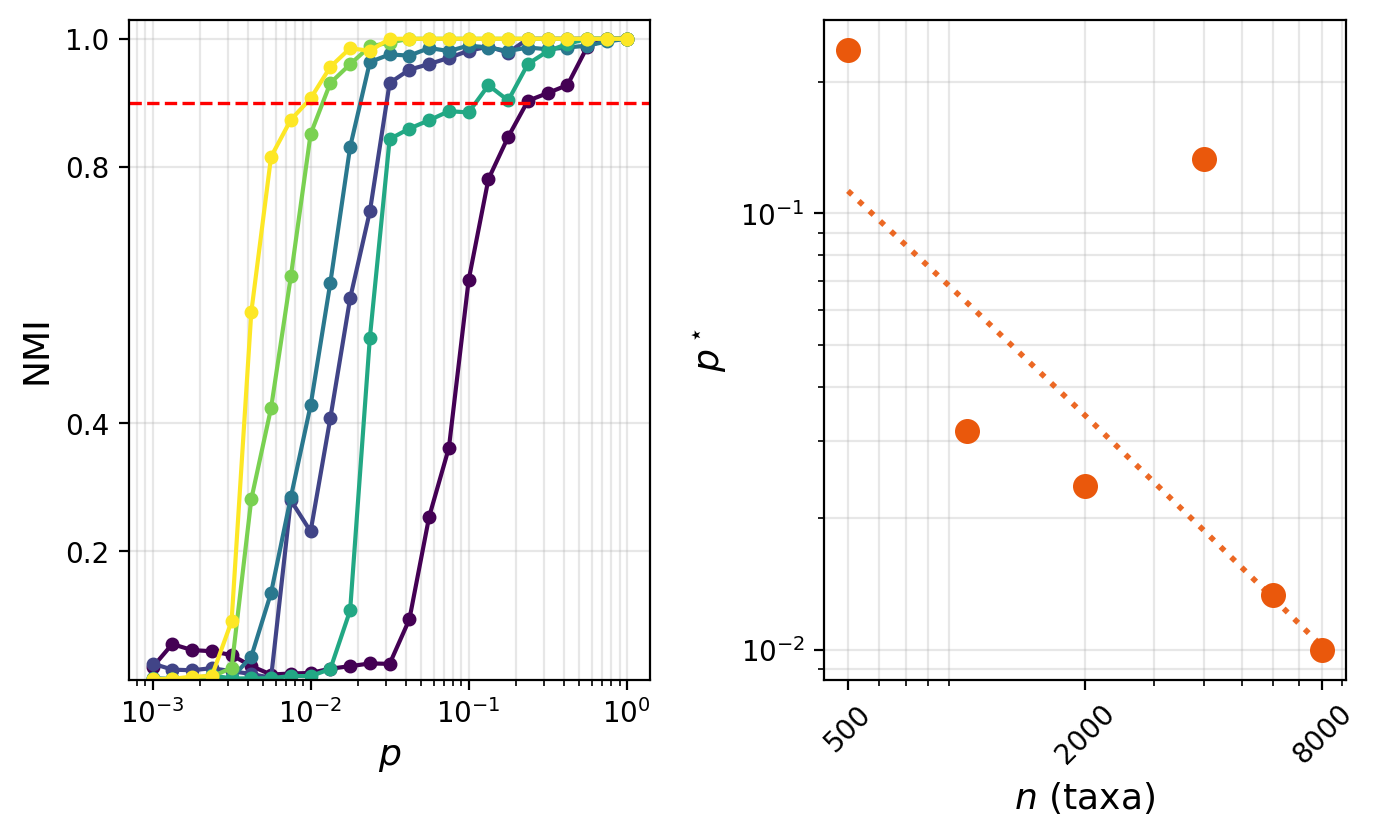
\includegraphics[width=\textwidth]{pstar_gen_kmeans_eta10.png}
    \end{subfigure}
    \hfill
    \begin{subfigure}[t]{0.49\textwidth}
        \captionsetup{singlelinecheck=false, justification=raggedright, skip=1pt}
        \subcaption{$\eta\approx15$}\label{fig:pstar_gen_eta15}
        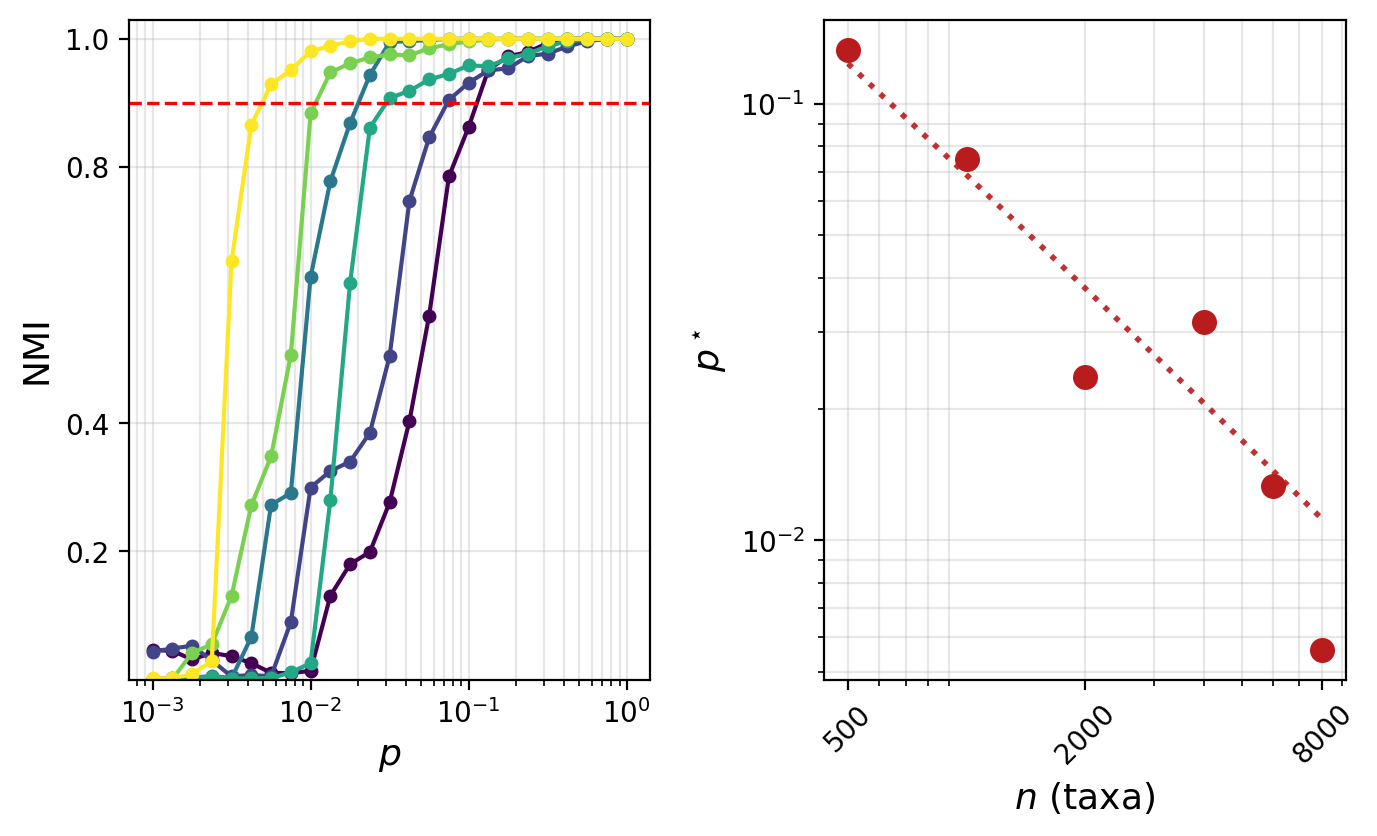
\includegraphics[width=\textwidth]{pstar_gen_kmeans_eta15.png}
    \end{subfigure}
    \caption{\textbf{Similarity route, simulated phylogenies.} Kingman trees carrying
    JC69 sequences, with $S$ estimated from the alignment rather than written down.
    The $\log m/m$ decay of \Cref{fig:pstar_synth} survives off-model tree shapes and
    per-entry estimation noise.}
    \label{fig:pstar_gen}
\end{figure}

     % §8  Empirical study                  (sec:empirical)

\newpage
\bibliography{references}

\newpage
%==============================================================================
%  Appendices
%==============================================================================
\appendix
% Appendices are \section's, so cleveref called every \Cref{app:*} "Section A"
% rather than "Appendix A" -- visible in the main text wherever a proof is
% deferred.  \crefalias retargets the section counter for everything below.
\crefalias{section}{appendix}
\crefalias{subsection}{appendix}
% Appendix A.  Proofs of the population spectral geometry.  The order lem:A-decomp ->
% prop:coherence -> lem:gap -> lem:A-decomp(iv) is load-bearing: lem:gap uses only the
% inequality lambda_2 <= m*beta_0, and clause (iv) then uses lem:gap's interlacing
% bound to force equality.  Reordering makes the identification circular.
\section{Proof of the spectral geometry}\label{app:comp1}

\noindent Every later appeal to a bounded population entry is to \eqref{eq:cfbm_floor}.
No range claim is made for $\hat S$: by \eqref{eq:sampling_estimator} its observed
off-diagonal entries equal $S_{ij}/p$, which exceed $1$ throughout the regime
$p=\Theta(\log m/m)$ of interest.

\noindent We first verify that the model of \Cref{def:cfbm} is realised at the root split.

\begin{proof}[Proof of \Cref{prop:cfbm}]
Under \Cref{asm:clock} the tree is ultrametric, $d_{ij}=2\tau_{ij}$, so \eqref{eq:similarity_gtr}
reads
\begin{equation}\label{eq:similarity_clock}
   S_{ij}=\exp\bigl(2\,\mathrm{tr}(Q)\,\tau_{ij}\bigr),
\end{equation}
and $S$ records the coalescence heights of $\mathcal{T}$, one entry per pair.

Let $i \in C_1$ and $j \in C_2$. Every path from $C_1$ to $C_2$ traverses the root, so
$\mathrm{MRCA}(i,j) = r$ and $\tau_{ij} = \tau_r$ for every cross-block pair; this is purely
topological. By \eqref{eq:similarity_clock} all cross-block entries then equal the single value
$\bze = \exp(2\,\mathrm{tr}(Q)\tau_r)$, which lies in $(0,1)$ because $\mathrm{tr}(Q)<0$ and
$\tau_r>0$.

Now let $i \ne j$ lie in the same clade, say $C_1$, with clade root $h_1$. Then $\mathrm{MRCA}(i,j)$ is
a descendant of $h_1$, so $\tau_{ij} \le \tau^{\max} \le \max(\tau_{h_1},\tau_{h_2}) < \tau_r$, the
last inequality strict because the two root branches have positive length. As $\mathrm{tr}(Q)<0$,
\eqref{eq:similarity_clock} is strictly decreasing in $\tau_{ij}$, so
$S_{ij} \ge \exp(2\,\mathrm{tr}(Q)\tau^{\max}) = \Sin^{\min} > \bze$. In the other direction,
$\mathrm{MRCA}(i,j)$ is a strict ancestor of both $i$ and $j$ for $i \ne j$, so $\tau_{ij}>0$ and
$S_{ij}<1$; taking the maximum over the finitely many pairs gives $\Smax<1$. Together with
$\tau_{ii}=0$, giving $S_{ii}=\exp(0)=1$, this is \eqref{eq:cfbm_floor} and the stated range. The block degrees in
\eqref{eq:block_forms} follow by summing the rows of $S$ within each block and adding the constant
cross-block contribution, $|C_2|\bze$ for a row of $C_1$ and $|C_1|\bze$ for a row of $C_2$.
\end{proof}

\noindent We next prove the spectral decomposition stated in \Cref{sec:bridging},
which the proof of \Cref{lem:gap} then uses.

\begin{proof}[Proof of \Cref{lem:A-decomp}(i)--(iii)]
For any $L=D-S$, $L\1=D\1-S\1=0$, so $0$ is an eigenvalue with
$v^{(1)}=\tfrac1{\sqrt m}\1_m$; no assumption on $S$ is needed. Every off-diagonal
entry of $S$ is at least $\bze>0$ by \eqref{eq:cfbm_floor}, so the similarity graph is
connected and $\lambda_1=0$ is simple.

\emph{Step heights.} Assume $\vv$ has the stated form with $c_1,c_2>0$. The
constraints $\norm{\vv}_2=1$ and $\langle v^{(1)},\vv\rangle=0$ give $|C_1|c_1=|C_2|c_2$,
hence
\[
   |C_1|\Bigl(\tfrac{|C_2|}{|C_1|}c_2\Bigr)^2+|C_2|c_2^2=1
   \;\Longrightarrow\;\tfrac{|C_2|m}{|C_1|}c_2^2=1
   \;\Longrightarrow\; c_2^2=\tfrac{|C_1|}{|C_2|m},\quad c_1^2=\tfrac{|C_2|}{|C_1|m}.
\]

\emph{Eigenpair verification.} Write $\vv=(c_1\1_{|C_1|},\,-c_2\1_{|C_2|})^\top$ with
$|C_1|c_1=|C_2|c_2$. The only structural input is that the diagonal sub-degrees of
\eqref{eq:block_forms} already carry the row sums of their own block,
$D_{C_1}=\operatorname{diag}(S_{C_1}\1_{|C_1|})+|C_2|\bze I_{|C_1|}$, so that
\begin{equation}\label{eq:block_annihilation}
   (D_{C_1}-S_{C_1})\1_{|C_1|}=|C_2|\bze\1_{|C_1|},\qquad(D_{C_2}-S_{C_2})\1_{|C_2|}=|C_1|\bze\1_{|C_2|},
\end{equation}
\emph{identically, for arbitrary symmetric $S_{C_1},S_{C_2}$}: no constancy of the diagonal
blocks is used, and the within-block floor of \eqref{eq:cfbm_floor} plays no role here.
Using the block form of $L$ with $J_{|C_1|\times|C_2|}\1_{|C_2|}=|C_2|\1_{|C_1|}$,
$J_{|C_2|\times|C_1|}\1_{|C_1|}=|C_1|\1_{|C_2|}$ and \eqref{eq:block_annihilation},
\[
   Lv^{(2)}=
   \begin{pmatrix}
     |C_2|\bze c_1\1_{|C_1|}+|C_2|\bze c_2\1_{|C_1|}\\[2pt]
     -|C_1|\bze c_1\1_{|C_2|}-|C_1|\bze c_2\1_{|C_2|}
   \end{pmatrix},
\]
which reduces to
$\bigl(|C_2|\bze(c_1+c_2)\1_{|C_1|},\,-|C_1|\bze(c_1+c_2)\1_{|C_2|}\bigr)^\top$. From
$|C_1|c_1=|C_2|c_2$, $|C_2|(c_1+c_2)=mc_1$ and $|C_1|(c_1+c_2)=mc_2$, so $Lv^{(2)}=m\bze\,\vv$: the pair
$(m\bze,\vv)$ is an eigenpair, which is claim~(ii).

\emph{The bound \eqref{eq:lambda2_upper}.} Since $\lambda_1=0$ is simple with
eigenvector $v^{(1)}$, the Courant--Fischer characterisation of the second
eigenvalue reads $\lambda_2=\min\{x^\top Lx:\ \norm{x}_2=1,\ x\perp v^{(1)}\}$. The
vector $\vv$ is admissible in that minimisation --- it is a unit vector and
$\langle v^{(1)},\vv\rangle=0$ by construction --- so
$\lambda_2\le\langle\vv,L\vv\rangle=m\bze\norm{\vv}_2^2=m\bze$.
\end{proof}

\noindent Nothing above forces $\lambda_2$ to \emph{equal} $m\bze$; that is an
ordering claim, and it is what \Cref{asm:margin} supplies in clause (iv), proved at
the end of this appendix after the interlacing bound it needs.

\begin{proof}[Proof of \Cref{prop:coherence}]
Substituting the Fiedler coordinates of \Cref{lem:A-decomp} into
\eqref{eq:coherence_definition},
\[
   \coh=\tfrac m2\max\Bigl\{\tfrac1m+c_1^2,\ \tfrac1m+c_2^2\Bigr\}
       =\tfrac m2\Bigl(\tfrac1m+\tfrac{|C_2|}{m|C_1|}\Bigr)
       =\tfrac12\Bigl(1+\tfrac{|C_2|}{|C_1|}\Bigr)=\tfrac{1+\eta}{2}. \qedhere
\]
\end{proof}

\begin{proof}[Proof of \Cref{lem:gap}]
The argument uses \Cref{asm:clock} and \Cref{prop:cfbm}, and only the
\emph{inequality} \eqref{eq:lambda2_upper}, $\lambda_2\le m\bze$ ---
not clause (iv) of \Cref{lem:A-decomp}, whose proof appeals to the interlacing step
below.
For $\lambda_3$, standard algebraic-connectivity interlacing gives
$\lambda_3(L)\ge\min\bigl(\lambda_2(L_{C_1}),\lambda_2(L_{C_2})\bigr)$, and applying
the Fiedler-eigenvalue formula to each clade Laplacian gives
$\lambda_2(L_{C_k})\ge|C_k|\,\Sin^{\min}$ for $k=1,2$, with $\Sin^{\min}$ the weakest
within-block similarity of \eqref{eq:cfbm_floor},
\begin{equation}\label{eq:lambda3_lower}
   \lambda_3\ \ge\ \min\bigl(\lambda_2(L_{C_1}),\lambda_2(L_{C_2})\bigr)
   \ \ge\ \min(|C_1|,|C_2|)\,\Sin^{\min}=m_{\min}\Sin^{\min},
\end{equation}
so $\Dlam=\lambda_3-\lambda_2\ge m_{\min}\Sin^{\min}-m\bze$. Using
$\Sin^{\min}=\rho+\bze$, which is \eqref{eq:margin_definition}, and
$m=m_{\min}(1+\eta)$,
\[
   \Dlam\ge m_{\min}(\rho+\bze)-(1+\eta)m_{\min}\bze
        =m_{\min}\rho-\eta\,m_{\min}\bze. \qedhere
\]
\end{proof}


\begin{proof}[Proof of \Cref{cor:tolerance}]
Positivity of the bound in \Cref{lem:gap} requires
$\eta<\Sin^{\min}/\bze$. The minimum within-block similarity is bounded by
the diameter, $\Sin^{\min}\ge e^{-r(\mathcal T)}$, and the maximum cross-block
similarity by the subtree depth, $\bze\propto e^{-\mathcal O(h(\mathcal T))}$.
Substituting into $\eta<\Sin^{\min}/\bze$ gives \eqref{eq:eta_distance_bound};
the logarithmic scaling $r,h=\mathcal O(\log m)$ under Kingman yields
$\eta\le\mathcal O(e^{\mathcal O(\log m)})=\mathcal O(m^c)$.
\end{proof}

\noindent With \eqref{eq:lambda3_lower} in hand the inequality
\eqref{eq:lambda2_upper} can be closed.

\begin{proof}[Proof of \Cref{lem:A-decomp}(iv)]
Suppose $\lambda_2<m\bze$. Then $m\bze$, an eigenvalue of $L$ by
\Cref{lem:A-decomp}(ii) and equal to neither $\lambda_1=0$ nor $\lambda_2$, satisfies
$m\bze\ge\lambda_3$. The interlacing bound \eqref{eq:lambda3_lower} gives
$\lambda_3\ge m_{\min}\Sin^{\min}$, so this forces $m_{\min}\Sin^{\min}\le m\bze$.
With $m=m_{\min}(1+\eta)$, \Cref{asm:margin} reads $\Sin^{\min}>(1+\eta)\bze$, i.e.\
$m_{\min}\Sin^{\min}>m\bze$ --- a contradiction. Hence $\lambda_2=m\bze$, and then
$\lambda_3\ge m_{\min}\Sin^{\min}>m\bze=\lambda_2$ shows $\lambda_2$ is simple, so
$\vv$ is the Fiedler vector up to sign.
\end{proof}
         % App A  spectral geometry
% Appendix B.  Proof of lem:B-bernstein: the operator-norm error of the sampled Laplacian,
% obtained from the row norms of S rather than from the coherence -- which is why mu(U)
% does not enter the sampling rate.
\section{Proof of the Laplacian sampling error}\label{app:comp2}

We prove \Cref{lem:B-bernstein} by bounding
$\opnorm{\EL}\le\opnorm{\ED}+\opnorm{\ES}$, where $\ES=\hat S-S$ and
$\ED=\hat D-D$. The only structural fact needed is the entry range
\eqref{eq:cfbm_floor}. By \eqref{eq:sampling_estimator} the diagonal is observed exactly,
$\hat S_{ii}=S_{ii}=1$, so it carries no noise and only off-diagonal pairs enter the
sums below; on those $S_{ij}\le\Smax<1$, giving
\begin{equation}\label{eq:row_norm_trivial}
   \max_i\sum_{j\ne i}S_{ij}^2\;\le\;(m-1)\,\Smax^2\;<\;m\,\Smax^2 .
\end{equation}

\begin{proof}[Proof of \Cref{lem:B-bernstein}]
\emph{Bounding $\opnorm{\ES}$.} Write $\ES=\sum_{i<j}Z^{(ij)}$, where $Z^{(ij)}$
is supported on the symmetric off-diagonal pair $(i,j)$ with value
$(\tfrac1p\Omega_{ij}-1)S_{ij}$;
the summands are independent and mean zero. The scale is
$\opnorm{Z^{(ij)}}\le\max(\tfrac1p-1,1)S_{ij}\le\Smax/p=:R$. For the variance proxy,
$\E[(Z^{(ij)}_{ij})^2]=\tfrac{p(1-p)}{p^2}S_{ij}^2\le\tfrac1pS_{ij}^2$, so by
\eqref{eq:row_norm_trivial},
\[
   \sigma^2\le\tfrac1p\max_i\sum_{j\ne i}S_{ij}^2\le\tfrac1p m\Smax^2 .
\]
Matrix Bernstein \cite{tropp2012userfriendly},
$\Prob(\opnorm{\ES}\ge t)\le2m\exp(\tfrac{-t^2/2}{\sigma^2+Rt/3})$, gives in the
variance-dominated regime, with probability $1-\epsilon$,
$\opnorm{\ES}\le2\Smax\sqrt{m\ln(2m/\epsilon)/p}$.

\emph{Bounding $\opnorm{\ED}$.} $\ED$ is diagonal with
$(\ED)_{ii}=\sum_{j\ne i}(\tfrac1p\Omega_{ij}-1)S_{ij}$; a scalar Bernstein with
$\sigma_D^2\le\tfrac1p mS_{\max}^2$ and $R_D=\Smax/p$ gives
$\opnorm{\ED}\lesssim\Smax\sqrt{m\ln(2m/\epsilon)/p}$.

\emph{Synthesis.} The two terms are now of the same order, so
\[
   \opnorm{\EL}\le\opnorm{\ES}+\opnorm{\ED}\le\tilde C\sqrt{\frac{m\log m}{p}},
\]
with $\tilde C$ absorbing $\Smax$ and absolute constants. The bound is uniform in
$\eta$: the imbalance enters the argument only through the gap $\Dlam$ this noise
is compared against, not through the noise itself.
\end{proof}
  % App B  Laplacian sampling error
% Appendix C.  Proofs of the entry-wise perturbation chain: Neumann series, per-node
% concentration, and the discarded remainder that confines the argument to the
% strong-signal regime.
\section{Proof of the entry-wise perturbation}\label{app:comp3}

\subsection{Neumann decomposition (proof of \Cref{lem:neumann})}\label{app:comp3a}

Write $\hat L=L+\EL$ and $\vvh=\vv+w$, and expand $w$ into a resolvent power series
in $\EL$ \cite{eldridge2017unperturbed}.

\begin{lemma}[Exact Neumann decomposition]\label{lem:C-series}
Define
\[
   w^{(1)}=\sum_{\ell\ne2}\frac{-\langle v^{(\ell)},\EL\vv\rangle}
        {\lambda_\ell-\hat\lambda_2}v^{(\ell)},
   \quad
   w^{(2)}=\sum_{\ell\ne2}\frac{-\langle v^{(\ell)},\EL w\rangle}
        {\lambda_\ell-\hat\lambda_2}v^{(\ell)}+\langle v^{(2)},w\rangle v^{(2)}.
\]
Then $w=w^{(1)}+w^{(2)}$ exactly, and under $\opnorm{\EL}<\Dlam$ this is the
resolvent series $w=\sum_{k\ge1}(-1)^k(\Dlam^{-1}\Pi\EL)^k\vv$.
\end{lemma}
\begin{proof}
From $\hat L\vvh=\hat\lambda_2\vvh$ and $L\vv=\lambda_2\vv$,
$(L-\hat\lambda_2I)w=(\hat\lambda_2-\lambda_2)\vv-\EL\vv-\EL w$. Projecting onto
$v^{(\ell)}$ ($\ell\ne2$), using $\langle v^{(\ell)},\vv\rangle=0$, gives
$\langle v^{(\ell)},w\rangle=(-\langle v^{(\ell)},\EL\vv\rangle-\langle
v^{(\ell)},\EL w\rangle)/(\lambda_\ell-\hat\lambda_2)$. Expanding
$w=\sum_\ell\langle v^{(\ell)},w\rangle v^{(\ell)}$ and separating the $\ell=2$
component recovers the decomposition; iterating on $\EL w$ under $\opnorm{\EL}<\Dlam$
yields the convergent series.
\end{proof}

\begin{lemma}[Entry-level first-order bound]\label{lem:C-first}
Provided $\opnorm{\EL}<\Dlam$, for every node $i$,
\begin{equation}
   |w^{(1)}_i|\le\frac{|(\EL\vv)_i|+\opnorm{\EL}\,|\vv_i|}{\Dlam-\opnorm{\EL}}.
\end{equation}
\end{lemma}
\begin{proof}
By Weyl's inequality $|\lambda_\ell-\hat\lambda_2|\ge\Dlam-\opnorm{\EL}$ for
$\ell\ne2$. Factoring the denominator,
$|w^{(1)}_i|\le|(P_\perp\EL\vv)_i|/(\Dlam-\opnorm{\EL})$ with
$P_\perp=I-\vv(\vv)^\top$. Since $P_\perp x=x-\langle\vv,x\rangle\vv$ and
$|\langle\vv,\EL\vv\rangle|\le\opnorm{\EL}\norm{\vv}_2^2=\opnorm{\EL}$,
$|(P_\perp\EL\vv)_i|\le|(\EL\vv)_i|+\opnorm{\EL}|\vv_i|$.
\end{proof}

\begin{remark}[Asymmetric correction in the constant block model]\label{rem:C-asym}
The correction $\opnorm{\EL}|\vv_i|$ equals $\opnorm{\EL}c_1$ for $i\in C_1$ and
$\opnorm{\EL}c_2$ for $i\in C_2$. For the binding clade $C_2$ this is
$\opnorm{\EL}/\sqrt{m\eta}$, strictly sub-dominant to the recovery target $c_2$
when $\opnorm{\EL}\ll\Dlam$. Throughout \Cref{app:comp3b} we therefore use the
leading-order simplification $|w^{(1)}_i|\lesssim|(\EL\vv)_i|/\Dlam$ for $i\in C_2$.
\end{remark}

\subsection{Per-node Bernstein concentration}\label{app:comp3b}

Under the leading-order simplification of \Cref{rem:C-asym} the entry-wise error
at node $i$ is governed by the scalar $(\EL\vv)_i$, which we now represent as a
sum of independent increments and concentrate.

\begin{lemma}[Laplacian increment representation]\label{lem:C-inc}
For every node $i$, $(\EL\vv)_i=\sum_{j\ne i}X_{ij}$ with
$X_{ij}=(\tfrac{\omega_{ij}}{p}-1)S_{ij}(\vv_i-\vv_j)$ independent and mean zero.
\end{lemma}
\begin{proof}
With $(\ES)_{ij}=(\omega_{ij}/p-1)S_{ij}$, $(\EL)_{ii}=\sum_{k\ne i}(\ES)_{ik}$ and
$(\EL)_{ij}=-(\ES)_{ij}$, so
$(\EL\vv)_i=\sum_{k\ne i}(\ES)_{ik}\vv_i-\sum_{j\ne i}(\ES)_{ij}\vv_j
=\sum_{j\ne i}(\ES)_{ij}(\vv_i-\vv_j)$.
\end{proof}

\begin{proposition}[Within-block terms vanish]\label{prop:C-within}
Under \Cref{def:cfbm}, $\vv$ is constant on each clade (\Cref{lem:A-decomp}), so
$X_{ij}=0$ for within-block pairs; only cross-block pairs survive:
$(\EL\vv)_i=\sum_{j\in C_1}X_{ij}$ for $i\in C_2$, and
$(\EL\vv)_i=\sum_{j\in C_2}X_{ij}$ for $i\in C_1$.
\end{proposition}

\begin{proposition}[Per-node variance]\label{prop:C-var}
Under \Cref{def:cfbm} and the observation model \eqref{eq:sampling_estimator}, using
$(c_1+c_2)^2=m/(|C_1||C_2|)=(1+\eta)^2/(m\eta)$,
\begin{equation}
   \sigma_2^2:=\operatorname{Var}\bigl((\EL\vv)_i\bigr)\big|_{i\in C_2}
   =\frac{(1-p)(1+\eta)\bze^2}{\eta\,p},
   \qquad
   \sigma_1^2=\frac{(1-p)(1+\eta)\bze^2}{p}=\eta\,\sigma_2^2,
\end{equation}
so clade $C_2$ has strictly smaller per-node variance;
$\sigma_2^2=(1-p)\rhotil/p$ with $\rhotil=(1+\eta)\bze^2/\eta$.
\end{proposition}
\begin{proof}
For $i\in C_2$ each of the $|C_1|$ surviving terms has $S_{ij}=\bze$ and
$|\vv_i-\vv_j|=c_1+c_2$, so $\sigma_2^2=\tfrac{1-p}{p}(c_1+c_2)^2|C_1|\bze^2$;
substituting $|C_1|=m/(1+\eta)$ and $(c_1+c_2)^2=(1+\eta)^2/(m\eta)$ gives the stated
value. Clade $C_1$ follows symmetrically, with its $|C_2|$ cross-block terms.
\end{proof}

\begin{proof}[Proof of \Cref{lem:pernode}]
By \Cref{lem:C-inc,prop:C-within}, for $i\in C_2$ the quantity
$(\EL\vv)_i=\sum_{j\in C_1}X_{ij}$ is a sum of independent, mean-zero summands with
$|X_{ij}|\le\bze(c_1+c_2)/p=R_2$ and total variance $\sigma_2^2$
(\Cref{prop:C-var}). Bernstein's inequality for bounded independent summands gives
the stated two-term deviation bound at confidence $1-\delta$. In the
variance-dominated regime $p=\Theta(\log m/m)$ the linear term is of lower order,
and a union bound over the $m$ nodes at $\delta=\delta_0/m$ yields
\eqref{eq:concentration-bound}.
\end{proof}

\begin{proposition}[Clade $C_2$ is binding]\label{prop:C-bind}
Under \Cref{lem:A-decomp}, $\min_i|\vv_i|=|c_2|$, attained on the larger clade $C_2$. The
per-node condition $|(\EL\vv)_i|<\Dlam|\vv_i|$ requires
$p>8m(1+\eta)\bze^2\log m/\Dlam^2$ on $C_2$ (the clade-$C_1$ condition carries an extra
$1/\eta$), so since $\eta\ge1$, clade $C_2$ binds.
\end{proposition}
\begin{proof}
Squaring $\sqrt{8\sigma_2^2\log m}<\Dlam c_2$ and substituting $\sigma_2^2$ with
$c_2^2=1/(m\eta)$: the $\eta$ cancels, giving
$p>8m(1+\eta)\bze^2\log m/\Dlam^2$. Clade $C_1$ follows with $c_1^2=\eta/m$.
\end{proof}

\begin{corollary}[Per-node recovery condition]\label{cor:C-cond}
If $|w_i|<\min_i|\vv_i|$ for all $i$ then
$\operatorname{sign}(\vvh)=\operatorname{sign}(\vv)$. Combining
\Cref{lem:pernode,prop:C-bind} with the gap bound
$\Dlam\ge m(\rho-\eta\bze)/(1+\eta)$ (\Cref{lem:gap}) yields
\begin{equation}\label{eq:per-node-p}
   p>\frac{8(1+\eta)^3\bze^2\log m}{m(\rho-\eta\bze)^2}
    =\Theta\!\left(\frac{\log m}{m}\right),
\end{equation}
which is the rate \eqref{eq:main_rate} of \Cref{thm:main-sim}. This computation is
Step~4 of the proof in \Cref{sec:outline}.
\end{corollary}

\subsection{The second-order remainder}\label{app:comp3c}

The bound below is the term discarded at Step~2 of \Cref{sec:outline}; it is
what restricts the argument to the strong-signal regime $\opnorm{\EL}\ll\Dlam$.

\begin{lemma}[Second-order negligibility]\label{lem:C-remainder}
$\norm{w^{(2)}}_\infty=O\!\bigl(\opnorm{\EL}^2/\Dlam^2\bigr)$.
\end{lemma}
\begin{proof}
By Davis--Kahan $\norm{w}_2\le\opnorm{\EL}/(\Dlam-\opnorm{\EL})$. Each coefficient
$b_\ell=-\langle v^{(\ell)},\EL w\rangle$ satisfies $|b_\ell|\le\opnorm{\EL}\norm{w}_2$,
and since $|\lambda_\ell-\hat\lambda_2|\ge\Dlam-\opnorm{\EL}$ each summand of
$w^{(2)}$ contributes $O(\opnorm{\EL}^2/\Dlam^2)$ in $\ell_\infty$; the $\vv$
component obeys $|\langle\vv,w\rangle|=O(\norm{w}_2^2)=O(\opnorm{\EL}^2/\Dlam^2)$.
\end{proof}
    % App C  entry-wise perturbation
% Appendix D.  Point: on this model the entry-wise route costs a factor m less in p than
% the Davis--Kahan route.
\section{The Neumann trick --- comparison with standard bounds}\label{app:compare}

The recovery criterion \eqref{eq:entrywise} constrains $w=\vvh-\vv$ in the
entry-wise sense, $\norm{w}_\infty<c_2$, where $c_2=\min_i|\vv_i|$ is the
entry-wise margin, attained on the binding clade $C_2$ with $c_2^2=1/(m\eta)$, while
the sampled-Laplacian noise satisfies $\opnorm{\EL}\le\tilde C\sqrt{m\log
m/p}$ (\Cref{lem:B-bernstein}). The two routes below bound the same $w$, differing
only in how they relate the entry-wise constraint to $\EL$.

\paragraph{The standard ($\ell_2$) route.} Davis--Kahan controls only the Euclidean
norm, $\norm{w}_2\le\opnorm{\EL}/(\Dlam-\opnorm{\EL})$. Because the criterion is in
the supremum norm, this must be transferred via $\norm{w}_\infty\le\norm{w}_2$;
imposing $\norm{w}_2<c_2$ and substituting the noise bound in the regime
$\opnorm{\EL}\ll\Dlam$ yields $p_{\mathrm{naive}}\gtrsim m^2\eta\log m/\Dlam^2$,
i.e.\ $\eta(1+\eta)^2\log m/(\rho-\eta\bze)^2$ after the gap bound of \Cref{lem:gap}.

\paragraph{The entry-wise (Neumann) route.} \Cref{lem:neumann} bounds each
coordinate directly, replacing $\opnorm{\EL}$ by the scalar $(\EL\vv)_i$ at the
tightest coordinate $i\in C_2$. This scalar is a sum of $O(m)$ independent mean-zero
contributions concentrating at $\sigma_2^2=(1-p)(1+\eta)\bze^2/(\eta p)$
(\Cref{prop:C-var}), smaller than $\opnorm{\EL}^2$ by a factor $m$; imposing
$|w_i|<c_2$ and the gap bound recovers the rate of \Cref{cor:C-cond}.

\begin{remark}[$\ell_2$ vs.\ entry-wise]\label{rem:E-compare}
Comparing the two rates gives
$p_{\mathrm{naive}}/p_{\mathrm{Neumann}}=\Theta\bigl(m\eta/((1+\eta)\bze^2)\bigr)$,
a $\Theta(m)$
reduction for fixed $\eta$. The saving originates at the noise level: the operator
norm $\opnorm{\EL}$ exceeds the individual increment $(\EL\vv)_i$ by
$\Theta(\sqrt m)$, and since $p$ enters both rates as $p^{-1}$ under a square root
this squares to $\Theta(m)$. Both rates carry $(\rho-\eta\bze)^{-2}$ and so
diverge together as $\rho-\eta\bze\to0$ (the boundary of \Cref{asm:margin}), but the
entry-wise rate stays within $p\le1$ over a region where $p_{\mathrm{naive}}$
already exceeds it, so it accommodates more imbalanced trees than the Euclidean
route admits.
\end{remark}
    % App D  Neumann trick vs. standard bounds

% Appendix E.  Which split the Fiedler rule picks on 1000 simulated trees with no
% sub-sampling -- the measurement behind the eta values the sweeps of §7 use.
\section{Which Split the Fiedler Rule Picks}\label{app:eta}

Two cohorts of 1000 trees, Kingman and birth--death, at $m=1000$ and $\ell=10^4$ under
\Cref{asm:gtr,asm:clock}, with no sub-sampling. The split is taken as \Cref{thm:main-sim}
prescribes: $k$-means on the Fiedler vector of $L(S)$. Per tree we record the imbalance of the
returned split, $\eta=|C_2|/|C_1|$ with $|C_1|\le|C_2|$, and whether that split is an edge of the true
tree. \Cref{fig:eta-hist} reports both, per cohort.

\begin{figure}[t]
    \centering
    \begin{subfigure}[t]{0.49\textwidth}
        \captionsetup{singlelinecheck=false, justification=raggedright, skip=1pt}
        \subcaption{Kingman}\label{fig:eta-king-ls}
        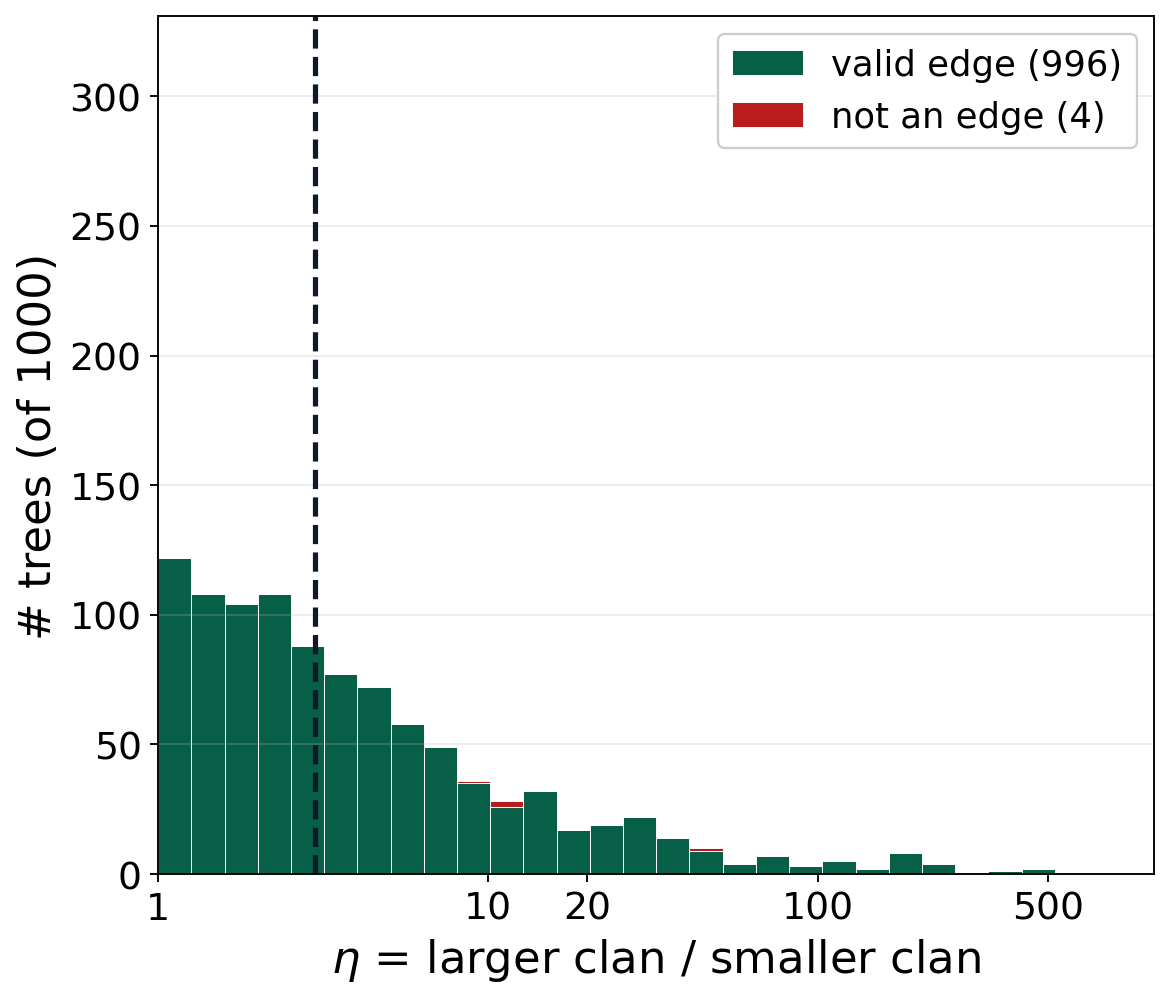
\includegraphics[width=\textwidth]{eta_hist_kingman_S.png}
    \end{subfigure}
    \hfill
    \begin{subfigure}[t]{0.49\textwidth}
        \captionsetup{singlelinecheck=false, justification=raggedright, skip=1pt}
        \subcaption{birth--death}\label{fig:eta-bd-ls}
        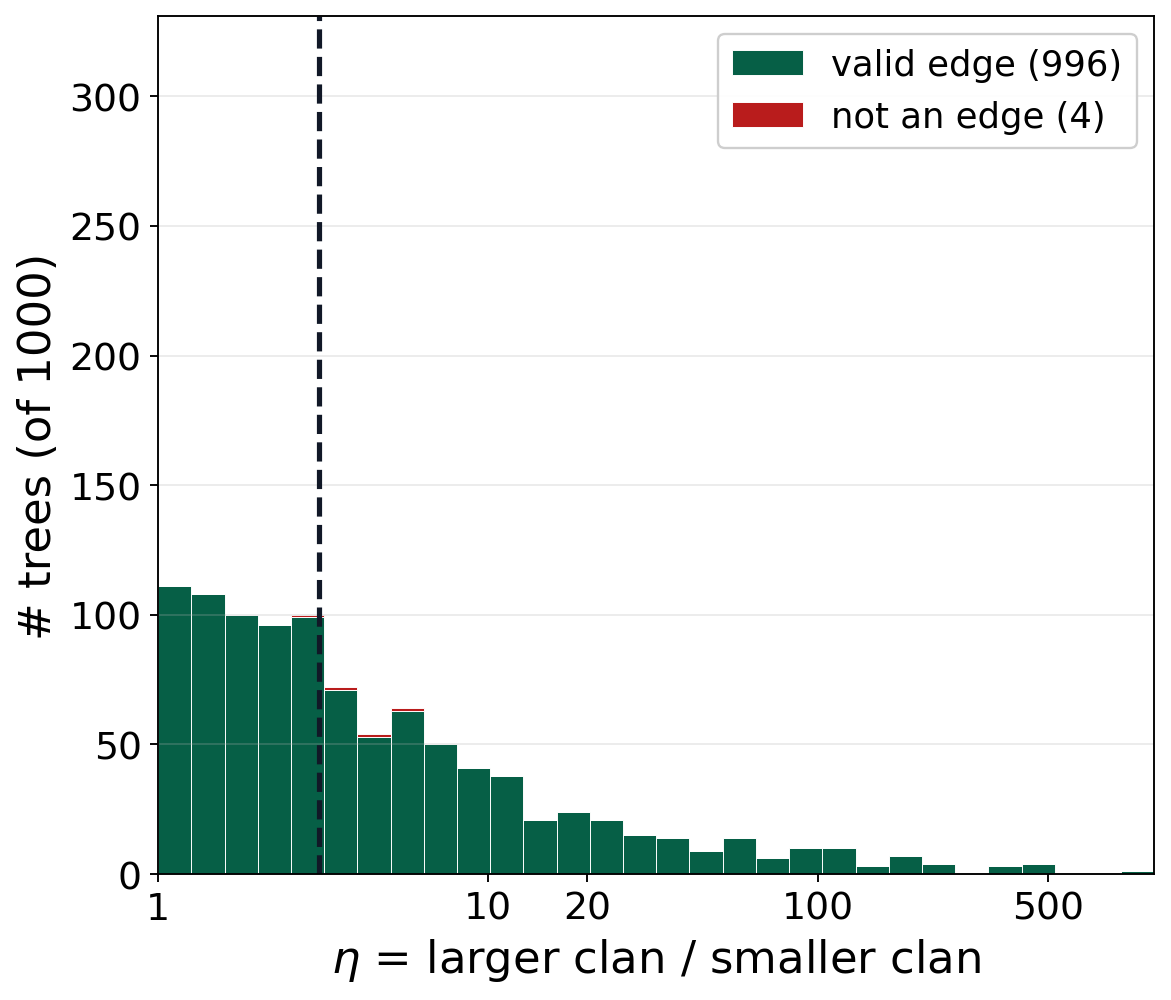
\includegraphics[width=\textwidth]{eta_hist_bd_S.png}
    \end{subfigure}

    \caption{\textbf{Imbalance of the returned split, 1000 trees per model.} Green is a
    genuine single-edge bipartition of the true tree, red is not; dashed line is the
    median. Both panels share bins and axes.}
    \label{fig:eta-hist}
\end{figure}

\begin{table}[t]
\centering
\caption{The Fiedler rule on both cohorts, 1000 trees each.}
\label{tab:eta-agreement}
\begin{tabular}{lrr}
\toprule
& Kingman & birth--death\\
\midrule
valid single-edge split & $996$  & $996$\\
median $\eta$           & $3.00$ & $3.08$\\
maximum $\eta$          & $499$  & $999$\\
\bottomrule
\end{tabular}
\end{table}

\noindent Two things follow from \Cref{tab:eta-agreement}, and both bear on how \Cref{sec:empirical}
reports its sweeps.

\begin{enumerate}[leftmargin=2em, itemsep=3pt, topsep=3pt]
\item \textbf{The rule returns an edge of the tree essentially always} --- $99.6\%$ on both
      cohorts --- which is \Cref{thm:stdr-split} measured under estimation noise rather than on the
      population matrix.
\item \textbf{The imbalance it returns spans three orders of magnitude}, with a median near $3$ and
      a maximum of $499$ on Kingman and $999$ on birth--death. Since $\eta$ enters
      \eqref{eq:main_rate} cubically, a sweep that pools trees across this range reports an average
      over recovery problems of very different difficulty. This is why \Cref{sec:empirical}
      stratifies by $\eta$ rather than pooling.
\end{enumerate}
             % App E  which split the Fiedler rule picks

\end{document}
